\documentclass[12pt,twoside,singlespace]{article}
\pagestyle{plain}

\usepackage{array, paralist, enumerate, amsmath, amsthm, amsfonts, amssymb, color, mathrsfs,comment}
%\usepackage{times}
\usepackage{geometry}
\usepackage{framed}
\usepackage{hyperref}
\usepackage{graphicx}
\usepackage{epstopdf}

\usepackage{tikz}
\usepackage{tkz-graph}
\usetikzlibrary{arrows,%
                shapes,positioning}

\definecolor{DarkBlue}{rgb}{0,0,0.8} 
\definecolor{DarkGreen}{rgb}{0,0.5,0.0} 
\definecolor{DarkRed}{rgb}{0.9,0.0,0.0} 

\usepackage[T1]{fontenc}
\usepackage[latin1]{inputenc}
%\usepackage[inline]{showlabels}

\numberwithin{equation}{section}
\newtheorem{thm}[equation]{Theorem}
\newtheorem{lem}[equation]{Lemma}
\newtheorem{cor}[equation]{Corollary}
\newtheorem{prop}[equation]{Proposition}

\theoremstyle{definition}
\newtheorem{definition}[equation]{Definition}
\newtheorem{ex}[equation]{Example}	
\newtheorem{remark}[equation]{Remark}
\newtheorem{prob}{Problem}
\newtheorem{construction}[equation]{Construction}

\newcommand{\BB}{\mathbf{B}}
\newcommand{\ZZ}{\mathbf{Z}}
\newcommand{\NN}{\mathbf{N}}
\newcommand{\RR}{\mathbf{R}}
\newcommand{\QQ}{\mathbf{Q}}
\newcommand{\CC}{\mathbf{C}}
\newcommand{\FF}{\mathbf{F}}
\newcommand{\N}{N}
\newcommand{\po}[2]{\mathfrak{po}^{#1|#2}}
\newcommand{\on}{\operatorname}
\newcommand{\ra}{\rightarrow}
\newcommand{\ul}{\underline}
\newcommand{\ol}{\overline}
\newcommand{\nin}{\noindent}

\newcommand{\simple}{\text{simple}}
\newcommand{\Img}{\on{Im}}
\newcommand{\con}{\on{Con}}
\newcommand{\dash}{\on{Dash}}

\geometry{verbose,letterpaper,tmargin=1in}

\newcommand{\Q}{\overline{q}}
\newcommand{\w}{\on{weight}}

\newcommand{\val}{\on{Val}}
\newcommand{\smon}{\mathbf{SMon}}
\newcommand{\clif}{\on{clif}}
\newcommand{\cl}{\mathbf{Cl}}
%\newcommand{\mov}[2]{\on{mov}_{#2}(#1)}
\newcommand{\inc}{\on{inc}}
\newcommand{\cut}[4]{#1 = #2 \amalg_{#4} #3}
\newcommand{\cutr}[3]{#1 \amalg_{#3} #2}
%\newcommand{\piece}[3]{#1(#2|#3)}
\newcommand{\piece}[3]{#1_{#3}}
\newcommand{\wt}{\on{wt}}

\newcommand{\com}[1]{\textcolor{red}{$[\star \star \star$ #1 $\star \star \star]$}}

%%%%%%%%%%%%%%%%%%%%%%%%%%%%%% LyX specific LaTeX commands.
%% Bold symbol macro for standard LaTeX users
\providecommand{\boldsymbol}[1]{\mbox{\boldmath $#1$}}

%%%%%%%%%%%%%%%%%%%%%%%%%%%%%% User specified LaTeX commands.
\renewcommand{\vec}[1]{\mathbf{#1}}

%\renewcommand{\labelenumi}{(\alph{enumi})}
%\renewcommand{\labelenumii}{(\roman{enumii})}

%\usepackage{babel}

\title{Strucutral Theory of 2D Adinkras}
\author{Kevin Iga and Yan X Zhang}

\begin{document}

\pagestyle{plain}

\maketitle

\begin{abstract}
Adinkras are combinatorial objects developed to study supersymmetry representations. Most of the work so far on Adinkras apply to $1$-dimensional supersymmetry; in this paper, we give formal definitions and structural theorems for \emph{$2$-d Adinkras} to study $2$-dimensional supersymmetry. We show that the natural definitions we want (products, quotients, etc.) behave unexpectedly well, having a nice interplay with the classical theory of \emph{switching graphs}. Our main result is settling a conjecture of H\"ubsch, which helps us understand most of the structure of $2$-d Adinkras. The methods are mostly self-contained.
\end{abstract}

\section{Preliminaries}

\subsection{$1$-d Adinkras}
Adinkras in \com{[references]} will be referred to as $1$-d Adinkras in this paper, since they relate to supersymmetry in $1$ dimension.  We will review a definition of $1$-d Adinkras now.

\begin{definition}[$1$-d Adinkras]
Let $n$ be a non-negative integer.  A \emph{$1$-d Adinkra} with $n$ colors is $(V,E,c,\mu,h)$ where
\begin{itemize}
\item $(V,E)$ is a finite undirected graph (called the \emph{underlying graph} of the Adinkra) with vertex set\footnote{In \com{[Reference]}, there is also a bipartition of the vertices, where some vertices are represented by open circles and called bosons, and other vertices are represented by filled circles and called fermions.  This is not necessary to include in our definition, because the bipartition can be obtained directly from the grading.}
 $V$ and edge set $E\subset V\times V$,
\item $c:E\to \{1,\ldots,n\}$ is a map called the \emph{coloring},
\item $\mu:E\to \ZZ_2=\{0,1\}$ is a map called the \emph{dashing},
\item $h:V\to\ZZ$ is a map called the \emph{grading}.
\end{itemize}

These are required to satisfy the following:
\begin{enumerate}
\item If $(v,w)\in E$, then $(w,v)\in E$.  Furthermore, $c(v,w)=c(w,v)$ and $\mu(v,w)=\mu(w,v)$.  Intuitively, the edges are undirected.
\item For every $v\in V$ and $c\in \{1,\ldots,n\}$, there exist exactly one $w\in V$ so that $(v,w)\in E$ and $c(v,w)=c$.
\item If $c_1$, $c_2\in \{1,\ldots,n\}$ with $c_1\not=c_2$, and $v\in V$, then there exist $w$, $x$, and $y\in V$ so that $(v,w)$, $(w,x)$, $(x,y)$, and $(y,v)\in E$, and $c(v,w)=c(x,y)=c_1$ and $c(w,x)=c(y,v)=c_2$ and $\mu(v,w)+\mu(w,x)+\mu(x,y)+\mu(y,v)\equiv 1\pmod{2}$.  We call $\mu$ \emph{admissible} if this last condition holds for every $v$, $w$, $x$ and $y$ that satisfy the above.

\com{ I like this definition better, which I'll need later for the word ``parity.'' Merge/pick from the two as you wish. -Y}
 Given a cycle $C$ given by vertices $(v_0,\ldots,v_k)$ in an Adinkra with dashing function $\mu$, the \emph{parity of $\mu$ on $C$} is the sum
\[\sum_{i=0}^{k-1} \mu(v_i,v_{i+1})\pmod{2}.\]
Using this language, an \emph{admissable} dashing is exactly one where the parity on all $2$-colored $4$-cycles are $1 \pmod{2}$.

\item If $(v,w)\in E$, then $|h(v)-h(w)|=1$.
\end{enumerate}

Figure~\ref{fig:1d-examples} give examples of 1-d Adinkras.
\end{definition}

\begin{figure}
\begin{center}
\begin{tabular}{cc}
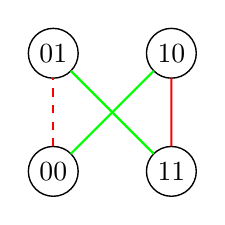
\begin{tikzpicture}[scale=0.15]
\SetUpEdge[labelstyle={draw}]
\Vertex[x=10,y=0]{11}
\Vertex[x=10,y=10]{10}
\Vertex[x=0,y=10]{01}
\Vertex[x=0,y=0]{00}
\Edge[color=green](00)(10)
\Edge[color=red, style=dashed](00)(01)
\Edge[color=red](10)(11)
\Edge[color=green](01)(11)
\end{tikzpicture}
& 
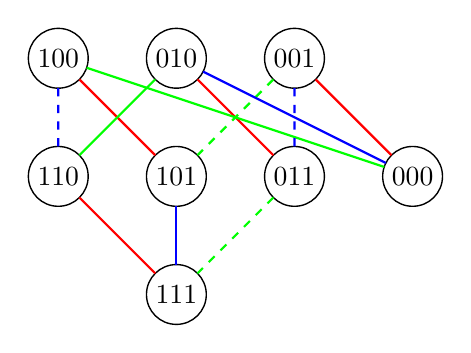
\begin{tikzpicture}[scale=0.15]
%\SetVertexNormal
\SetUpEdge[labelstyle={draw}]
\Vertex[x=0,y=0]{111}
\Vertex[x=0,y=10]{101}
\Vertex[x=0,y=20]{010}
\Vertex[x=20,y=10]{000}
\Vertex[x=-10,y=10]{110}
\Vertex[x=10,y=10]{011}
\Vertex[x=-10,y=20]{100}
\Vertex[x=10,y=20]{001}
\Edge[color=red](100)(101)
\Edge[color=red](000)(001)
\Edge[color=red](010)(011)
\Edge[color=red](110)(111)
\Edge[color=green](000)(100)
\Edge[color=green, style=dashed](001)(101)
\Edge[color=green](010)(110)
\Edge[color=green, style=dashed](011)(111)
\Edge[color=blue](000)(010)
\Edge[color=blue, style=dashed](001)(011)
\Edge[color=blue, style=dashed](100)(110)
\Edge[color=blue](101)(111)
\end{tikzpicture}
\\
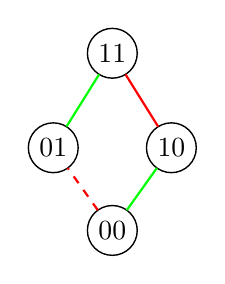
\begin{tikzpicture}[scale=0.15]
\SetUpEdge[labelstyle={draw}]
\Vertex[x=5,y=15]{11}
\Vertex[x=10,y=7]{10}
\Vertex[x=0,y=7]{01}
\Vertex[x=5,y=0]{00}
\Edge[color=green](00)(10)
\Edge[color=red, style=dashed](00)(01)
\Edge[color=red](10)(11)
\Edge[color=green](01)(11)
\end{tikzpicture}
&
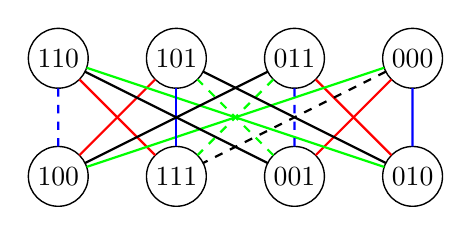
\begin{tikzpicture}[scale=0.15]
%\SetVertexNormal
\SetUpEdge[labelstyle={draw}]
\Vertex[x=0,y=0]{111}
\Vertex[x=0,y=10]{101}
\Vertex[x=20,y=0]{010}
\Vertex[x=20,y=10]{000}
\Vertex[x=-10,y=10]{110}
\Vertex[x=10,y=10]{011}
\Vertex[x=-10,y=0]{100}
\Vertex[x=10,y=0]{001}
\Edge[color=red](100)(101)
\Edge[color=red](000)(001)
\Edge[color=red](010)(011)
\Edge[color=red](110)(111)
\Edge[color=green](000)(100)
\Edge[color=green, style=dashed](001)(101)
\Edge[color=green](010)(110)
\Edge[color=green, style=dashed](011)(111)
\Edge[color=blue](000)(010)
\Edge[color=blue, style=dashed](001)(011)
\Edge[color=blue, style=dashed](100)(110)
\Edge[color=blue](101)(111)
\Edge[color=black](100)(011)
\Edge[color=black, style=dashed](000)(111)
\Edge[color=black](010)(101)
\Edge[color=black](110)(001)
\end{tikzpicture}
\end{tabular}
\caption{Examples of $1$-d Adinkras. In each picture, the grading function is represented by the relative vertical heights on the page.  \label{fig:1d-examples}}
\end{center}
\end{figure}

\subsection{The action of $\ZZ_2^n$ and the code}
Let $A$ be a $1$-d Adinkra with $n$ colors, with vertex set $V$.  For all $1\le i\le n$, define
\[q_i:V\to V\]
so that for all $v\in V$, $q_i(v)$ is the unique vertex joined to $v$ by an edge of color $i$.

\begin{definition}[Graph homomorphisms]
\label{defn:homomorphism}
A \emph{graph homomorphism} from a graph $(V_1,E_1)$ to a graph $(V_2,E_2)$ is a map $\phi:V_1\to V_2$ so that if $(v,w)\in E_1$ is an edge, then $(\phi(v),\phi(w))\in E_2$ is an edge.  If there is a coloring $c_1:E_1\to\{1,\ldots,n\}$ and a coloring $c_2:E_2\to\{1,\ldots,n\}$, we say that $\phi$ \emph{preserves colors} if $c_1(v,w)=c_2(\phi(v),\phi(w))$.  If $\phi$ is bijective, we say that it is a \emph{graph isomorphism}.
\end{definition}

\begin{prop}
\label{prop:qmap}
The map $q_i$ is a graph isomorphism from the underlying graph of $A$ to itself which preserves colors.  It is an involution and for all $i$, $j$, we have
\begin{equation}
q_i\circ q_j=q_j\circ q_i.\label{eq:commute}
\end{equation}
\end{prop}
\begin{proof}
The statement that $q_i$ is a graph homomorphism means that if $(v,w)$ is an edge in $A$, then so is $(q_i(v),q_i(w))$.  This follows from items 2 and 3 in the definition of an Adinkra above, using $j=c(v,w)$.

The fact that $q_i(q_i(v))=v$ for all $v\in V$ follows from item 2 in the definition.  This means that $q_i$ is an involution and in particular is an isomorphism.

The equation (\ref{eq:commute}) follows from item 3 of the definition when $i\not=j$ and is trivial when $i=j$.
\end{proof}

By combining the $q_1,\ldots, q_n$ maps, we can define an action of $\ZZ_2^n$ on the graph $(V,E)$ underlying the Adinkra in the following way:
\begin{definition}
The action of $\ZZ_2^n$ on the graph $(V,E)$ underlying the Adinkra is given on vertices by
\[(x_1,\ldots,x_n)v=q_1^{x_1}\circ\cdots\circ q_n^{x_n}(v).\]
\end{definition}

\begin{prop}
\label{prop:actioniso}
The above defines an action by graph isomorphisms that preserve colors.
\end{prop}
\begin{proof}
Acting on $v$ by $\vec{y}$ and then $\vec{x}$ gives
\begin{eqnarray*}
\vec{x}\vec{y}(v)
&=&q_1^{x_1}\circ\cdots\circ q_n^{x_n}\circ
q_1^{y_1}\circ\cdots\circ q_n^{y_n}(v)\\
&=&q_1^{x_1+y_1}\circ\cdots\circ q_n^{x_n+y_n}(v)
\end{eqnarray*}
by the commutativity shown in (\ref{eq:commute}), and where the exponents are taken modulo $2$, because each $q_i$ is an involution.  Therefore this is equal to
\[(\vec{x}+\vec{y})(v).\]

Proposition~\ref{prop:qmap} says that each $q_i$ is an isomorphism which preserves colors, and this action is a composition of such maps.
\end{proof}

\begin{definition}
A path is a finite sequence of edges of the form $((v_1,v_2),(v_2,v_3),\ldots,(v_{k-1},v_k))$.  The {\em color sequence} of the path is the sequence $(c(v_1,v_2),c(v_2,v_3),\ldots,c(v_{k-1},v_k))$.
\end{definition}

So if there is a path from $v$ to $w$ with color sequence $(i_1, \ldots, i_k)$, we have $w=q_{i_k}\circ \cdots\circ q_{i_1}(v)$.

\begin{prop}
\label{prop:colorpath}
Let $A$ be an Adinkra and let $v$ be a vertex of $A$.  Let $\sigma$ be a color sequence.  There exists a unique path in $A$ that starts at $v$ and has color sequence $\sigma$.
\end{prop}
\begin{proof}
This can be proved by induction on the length of $\sigma$, and using the fact that given a vertex $v_i$ of $A$, and a color $c_i$, there exists a unique vertex $v_{i+1}$ so that $(v_i,v_{i+1})$ is an edge of $A$ with color $c_i$.
\end{proof}

Now, define a map $s$ that takes a color sequence and returns an element of $\ZZ_2^n=\{0,1\}^n$ where the $i$-th coordinate is the number of times (modulo $2$) that color $i$ appears in the sequence. For example, $s(3,1,2,1) = 0110$.  Note that $s(\sigma)$ does not depend on the ordering of the color sequence $\sigma$.  This relates to paths in Adinkras because of the following:

\begin{prop}
\label{prop:colorendpath}
Let $A$ be an Adinkra.  Let $v$ be a vertex of $A$ and let $p$ be a path that begins at $v$.  Let $\sigma$ be the color sequence obtained from $p$.  Then the path $p$ ends at the vertex $s(\sigma)v$.
\end{prop}
\begin{proof}
If the color sequence is $\sigma=(i_1,\ldots,i_k)$, then the path $p$ ends at
$q_{i_k}\circ \cdots \circ q_{i_1}(v)$.  By the commutativity of the $q_i$, we can order them in non-decreasing order of $i_j$.  If any of the $q_i$ appear more than once, we use the fact that $q_i^2$ is the identity to reduce the number of $q_i$ modulo $2$.  The result is $s(\sigma)v$.
\end{proof}


\begin{cor}
\label{prop:pathands}
Let $A$ be an Adinkra.  Let $v$ be a vertex of $A$ and let $p$ and $p'$ be paths that begin at $v$.  Let $\sigma$ and $\sigma'$ be the color sequences obtained from $p$ and $p'$, respectively.  If $s(\sigma)=s(\sigma')$, then $p$ and $p'$ both end at the same point.
\end{cor}



\begin{definition}
Pick a vertex $v\in A$.  Define $C(A,v)$ to be the stabilizer of $v$ under this action of $\ZZ_2^n$.  Since it is a subgroup of $\ZZ_2^n$, $C(A,v)$ is a binary block code of length $n$.
\end{definition}

\begin{prop}
\label{prop:transitive}
The Adinkra $A$ is connected if and only if the $\ZZ_2^n$ action is transitive on the vertex set of $A$.
\end{prop}
\begin{proof}
Let $v$, $w$ be vertices of $A$.  If $A$ is connected, then there is a path in $A$ connecting $v$ to $w$.  Let $\sigma$ be the color sequence obtained from this path.  Then by Proposition~\ref{prop:colorendpath}, $s(\sigma)v=w$.

Conversely, suppose the action is transitive.  Let $v$ and $w$ be vertices of $A$.  Then there exists a $\vec{x}\in\ZZ_2^n$ so that $w=\vec{x}v$.  Write $\vec{x}=(x_1,\ldots,x_n)$ and construct a color sequence $\sigma$ by taking the $i$ for which $x_i=1$.  By Proposition~\ref{prop:colorpath}, there is a path starting at $v$ that has $\sigma$ as its color sequence.  By Proposition~\ref{prop:colorendpath}, this path ends at $s(\sigma)v=\vec{x}v=w$.
\end{proof}

\begin{prop}
If $A$ is connected, then the code $C(A,v)$ does not depend on $v$.
\end{prop}
\begin{proof}
Let $w\in V$.  By Proposition~\ref{prop:transitive}, there exists a $\vec{y}\in \ZZ_2^n$ so that $\vec{y} v=w$.

Let $\vec{x}\in \ZZ_2^n$.  The result follows from the sequence of equivalences:
\[\vec{x} w=w\Leftrightarrow \vec{x}\vec{y} v=\vec{y} v \Leftrightarrow \vec{y} \vec{x} v=\vec{y} v \Leftrightarrow \vec{x} v=v\]
\end{proof}

\begin{definition}
Given a connected Adinkra $A$, the \emph{code} for $A$, called $C(A)$, is defined to be $C(A,v)$, where $v$ is a vertex of $A$.
\end{definition}




\begin{prop}
\label{prop:paths}
Let $A$ be an Adinkra.  Let $v$ be a vertex of $A$ and let $p$ and $p'$ be paths that begin at $v$.  Let $\sigma$ and $\sigma'$ be the color sequences obtained from $p$ and $p'$, respectively.  The paths $p$ and $p'$ end at the same vertex if and only if 
\[s(\sigma)-s(\sigma')\in C(A).\]
\end{prop}

\begin{proof}
Suppose $p$ and $p'$ end at the same vertex.  Then by Proposition~\ref{prop:colorendpath},
\[s(\sigma)v=s(\sigma')v.\]
Then\footnote{Note that in this sequence of equations, $\ZZ_2^n$ is written additively but the group action is written multiplicatively.}
\[v=s(\sigma')^{-1}(s(\sigma)v)=(s(\sigma)-s(\sigma'))v.\]
Thus, $s(\sigma)-s(\sigma')\in C(A)$.

Conversely, suppose $s(\sigma)-s(\sigma')\in C(A)$.  Then by reversing the above argument,
\[s(\sigma)v=s(\sigma')v\]
and thus, by Proposition~\ref{prop:colorendpath}, $p$ and $p'$ end at the same vertex.
\end{proof}

\subsection{Quotients of graphs and Adinkras}
\label{sec:quotient}
As we have seen, $\ZZ_2^n$, and therefore subgroups of $\ZZ_2^n$, act on Adinkras (more precisely, the underlying graphs), and it will be important to understand quotients of Adinkras by codes.

\begin{prop}
Let $\Gamma=(V,E)$ be a graph, and suppose $C$ is a group that acts on $V$ via graph isomorphisms.  Then $C$ acts on the set of edges in the following manner: if $c\in C$ and $(v,w)\in E$, then $c(v,w)=(cv,cw)$.
\end{prop}
\begin{proof}
The fact that $(cv,cw)$ is an edge follows directly from the definition of graph isomorphism.

The fact that this is a group action follows from the fact that $c(c'(v,w))=(c(c'(v)),c(c'(w)))=((cc')v,(cc')w)=(cc')(v,w)$.
\end{proof}

\begin{definition}
Suppose $C$ is a group that acts on a graph $(V,E)$ via graph isomorphisms.  We say that this group action is distant if for every non-identity group element $c\in C$, and every vertex $v\in V$, every path from $v$ to $cv$ is of length greater than 2.
\end{definition}

\begin{construction}
If a group $C$ acts on a graph $\Gamma=(V,E)$ via graph isomorphisms, then we create a graph $\Gamma/C$ as follows: let the set of vertices be the orbit space $V/C$.  Edges in $\Gamma/C$ are pairs $(Cv,Cw)$ where there exist $c_1, c_2\in C$ so that $(c_1v,c_2h)$ is an edge in $E$.
\end{construction}

\begin{prop}
\label{prop:distiso}
If, in the previous construction, the group action is distant, then there is a bijection from $E/C$ to the set of edges in $\Gamma/C$.
\end{prop}
\begin{proof}
For every orbit $C(v,w)$ of $C$ on the set of edges of $\Gamma$, there is an edge $(Cv,Cw)$.  This is an edge in $\Gamma/C$ because $(v,w)$ is an edge in $\Gamma$.  This assignment is independent of the choice of representative $(v,w)$ from $C(v,w)$ above since if $(v',w')$ is another representative, then there is a group element $c\in C$ so that $v'=cv$ and $w'=cw$.  Then $v'\in Cv$ and $w'\in Cw$ so that $Cv'=Cv$ and $Cw'=Cw$.

To see that this assignment is surjective follows directly from the definition: for every edge in $\Gamma/C$, there is an edge $(v,w)$ in $\Gamma$ that gets sent to it.

Now to prove that this is injective, suppose $(v,w)$ and $(v',w')$ are edges in $\Gamma$ and suppose $(Cv,Cw)=(Cv',Cw')$.  Then there are group elements $c_1$ and $c_2\in C$ so that $c_1v=v'$ and $c_2w=w'$.  On the other hand, there is an edge $(c_1v,c_1w)=(v',c_1w)$.  So $(v',c_1w)$ and $(v',c_2w)=(v',w')$ are edges in the graph.  Then $c_2c_1^{-1}$ is a group element that sends $c_1w$ to $c_2w$ but we have just constructed a path of length 2 from $c_1w$ to $c_2w$.  Since the group action is distant, we know that $c_2c_1^{-1}=1$ so that $c_1=c_2$.  Therefore $(v',w')=c_1(v,w)$.
\end{proof}

\begin{prop}
\label{prop:quotient}
If a group $C$ acts on an Adinkra $A$ using graph isomorphisms that preserve colors, and if the action is distant, then the coloring descends to a coloring on $A/C$ that satisfies those properties of Adinkras that relate to colors and not to dashings or grading.  That is, let $E/C$ denote the set of edges of $A/C$ as defined in the construction.  Then
\begin{enumerate}
\item If $(Cv,Cw)$ is an edge in $A/C$, then $(Cw,Cv)$ is also an edge.  Furthermore, $c(Cv,Cw)=c(Cw,Cv)$.
\item For every $Cv\in V/C$ and $c\in \{1,\ldots,n\}$, there exist exactly one $Cw\in V/C$ so that $(Cv,Cw)\in E/C$ and $c(Cv,Cw)=c$.
\item If $c_1$, $c_2\in \{1,\ldots,n\}$ with $c_1\not=c_2$, and $Cv\in V/C$, then there exist $Cw$, $Cx$, and $Cy\in V/C$ so that $(Cv,Cw)$, $(Cw,Cx)$, $(Cx,Cy)$, and $(Cy,Cv)\in E/C$, and $c(Cv,Cw)=c(Cx,Cy)=c_1$ and $c(Cw,Cx)=c(Cy,Cv)=c_2$
\end{enumerate}
\end{prop}
\begin{proof}
Since Proposition~\ref{prop:distiso} says that the edges of $A/C$ can be identified with $E/C$, and since the action of $C$ preserves colors, we can define the coloring on $E/C$, and thus, on the edges of $A/C$.

Property 1 follows from the construction of the edges of $A/C$.

Now we prove Property 2.  Let $Cv\in V/C$ and $c\in\{1,\ldots,n\}$.  Since $A$ is an Adinkra, there is exactly one vertex $w\in V$ so that $(v,w)\in E$ and $c(v,w)=c$.  There is thus an edge $(Cv,Cw)$ in $A/C$ that has color $c$.  To show uniqueness, suppose there is an $x\in V$ so that $(Cv,Cx)$ is in $A/C$ with color $c$.  This means there are group elements $\alpha,\beta\in C$ so that $(\alpha v,\beta x)$ is an edge of $A$ of color $c$.  By acting by $\alpha^{-1}$, we see that without loss of generality, $\alpha=1$.  Because $A$ is an Adinkra, there is a unique edge from $v$ that has color $c$.  So $\beta x = w$.  Therefore $x\in Cw$.

Now we prove Property 3.  Let $c_1$ and $c_2$ be two different colors, and $Cv\in V/C$.  Since $A$ is an Adinkra, there are vertices $w$, $x$, and $y$ in $V$ so that $(v,w)$, $(w,x)$, $(x,y)$ and $(y,v)\in E$ and $c(v,w)=c(x,y)=c_1$ and $c(w,x)=c(y,v)=c_2$.  Then $Cw$, $Cx$, and $Cy$ are the requisite vertices in $V/C$ with the given property.
\end{proof}


\com{[Change notation?  Colors and codes are both $C$ and $c$...  Graphs are often $G$ but here they are $\Gamma$ because groups are often $G$.]}

\begin{prop}
If $A$ is an Adinkra and $C$ acts on $A$ via graph isomorphisms, then there is a map
\[\pi:A\to A/C\]
 that is a graph homomorphism.  If the action is distant and if $C$ acts preserving colors, then $\pi$ preserves colors.
\end{prop}
\begin{proof}
Let $\pi(v)=vC$.  If $(v,w)$ is an edge in $A$, then $\pi(v)=vC$ and $\pi(w)=wC$ are connected via an edge in $A/C$ because of the existence of the edges $(v,w)$.

If the action is distant and $C$ acts preserving colors, then by Proposition~\ref{prop:quotient}, $A/C$ has a well-defined coloring defined by the following: if $(v,w)$ is an edge, then the color of $(vC,wC)$ is the color of $(v,w)$.
\end{proof}


\subsection{Quotienting the cube by a code}



The following $1$-d Adinkra was defined in \com{[reference]}.
\begin{construction}
For any non-negative integer $n$, we have an Adinkra $I^n=(V,E,c,\mu,h)$ with
\begin{itemize}
\item $V=\ZZ_2^n=\{0,1\}^n$,
\item $E=\{(v,w)\,|\,\mbox{$v$ and $w$ differ in precisely one coordinate}\}$,
\item $c(v,w)$ is the coordinate where $v$ and $w$ differ,
\item $\mu(v,w)$ is the number of $1$s in $v$ before the coordinate $c(v,w)$, modulo $2$,
\item $h(v)=\wt(v)$ is the number of $1$s in $v$.
\end{itemize}
\end{construction}


\begin{definition}
Given $C$ a linear block code of length $n$, with all non-zero code words having weight greater than $2$, we can define an (edge-colored) graph $I^n/C$ as the orbit space of the action of $C\subset \ZZ_2^n$ on $I^n$ as a graph.
\end{definition}

Recall that $C$ acts via graph homomorphisms that preserve colors.  By Proposition~\ref{prop:quotient}, since code words are length at least $2$, the quotient $I^n/C$ makes sense as an edge-colored graph.

\begin{thm}
\label{thm:cubemodulocode}
If $A$ is a connected Adinkra, then there is a graph isomorphism from $I^n/C(A)$ to $A$ that preserves colors.
\end{thm}
\begin{proof}
Choose a vertex $\overline{0}$ in $A$.  Let
\[\phi:I^n\to A\]
\[\phi(x_1,\ldots,x_n)=(x_1,\ldots,x_n)\overline{0}\]
where we are using the action of $\ZZ_2^n$ on $A$ as described above.

To see that this is a graph homomorphism, let $(x_1,\ldots,x_n)\in\ZZ_2^n$ and let $(y_1,\ldots,y_n)$ be another vertex connected to $(x_1,\ldots,x_n)$ with an edge of color $i$.  Then $y_j=x_j$ for all $j\not=i$ and $y_i=1-x_i$.  Then $(y_1,\ldots,y_n)\overline{0}=q_1^{y_1}\cdots q_n^{y_n}(\overline{0}) =  q_1^{x_1}\cdots q_i^{1-x_i}\cdots q_n^{x_n}(\overline{0})=q_i(q_1^{x_1}\cdots q_n^{x_n}(\overline{0}))=q_i(x_1,\ldots,x_n)$.  So $\phi(x_1,\ldots,x_n)$ and $\phi(y_1,\ldots,y_n)$ are connected by an edge of color $i$.  Note that this also shows that the graph homomorphism preserves colors.

We now prove that $\phi$ is surjective.  Since $A$ is connected, $\ZZ_2^n$ acts transitively on the vertex set of $A$, and so for any vertex $v$ of $A$, there exists an element $\vec{x} \in\ZZ_2^n$ so that $\vec{x} \overline{0}=v$.  Then $v=\phi(\vec{x})$.

To prove the isomorphism from $I^n/C(A)$ to $A$, we consider the necessary and sufficient conditions for $\phi(\vec{x})=\phi(\vec{y})$ for $\vec{x}$, $\vec{y}\in \ZZ_2^n$.  The condition $\phi(\vec{x})=\phi(\vec{y})$ is equivalent to $\phi(\vec{x}-\vec{y})\overline{0}=\overline{0}$.  This is equivalent to saying $\vec{x}-\vec{y}\in C(A)$.  Thus, the map $\phi$ descends to $I^n/C(A)$ and gives an isomorphism.
\end{proof}

In \com{Reference ...}, it was proved that if $A$ is a connected Adinkra, then $C(A)$ is a doubly even code.  Furthermore, if $C$ is any doubly even binary block code of length $n$, then there is an Adinkra with $C(A)=C$.



\begin{lem}
\label{lem:uniqueiso}
Given connected $1$-d Adinkras $A$ and $B$ and vertices $a$ of $A$ and $b$ of $B$, there is at most one graph isomorphism from $A$ to $B$ that preserves colors and sends $a$ to $b$.
\end{lem}
\begin{proof}
Suppose $\phi:A\to B$ is a graph isomorphism that preserves colors and sends $a$ to $b$.

Let $v$ be a vertex of $A$. Since $A$ is connected, there is a path from $a$ to $v$.  This produces a color sequence $\sigma$.  Since $\phi$ is a graph isomorphism that preserves colors, $\phi$ sends this path to a path in $B$ starting from $b$ with the same color sequence.  By Proposition~\ref{prop:colorpath}, there is only one path in $B$ with this property.  The end of this path is $\phi(v)$.
\end{proof}


\com{Maybe delete this:}


\begin{definition}
Let 
$A_1=(V_1,E_1,c_1,\mu_1,h_{L1},h_{R1})$
and
$A_2=(V_2,E_2,c_2,\mu_2,h_{L2},h_{R2})$
be 2-Adinkras with $(p,q)$ colors.  A homomorphism from $A_1$ to $A_2$ is a graph homomorphism
\[\phi:(V_1,E_1)\to (V_2,E_2)\]
that preserves colors and so that:
\begin{itemize}
\item If $v\in V_1$ then $h_{1L}(v)=h_{2L}(\phi(v))$.
\item If $v\in V_1$ then $h_{1R}(v)=h_{2R}(\phi(v))$.
\end{itemize}
Note that there is no condition on the dashings $\mu_1$ and $\mu_2$.
\end{definition}

\subsection{[Possible things to use]}:

\com{@Kevin: I'm going to put things here that may be helpful. It isn't superimportant that they be from my papers; my goal is just to make this section compact but not weasel-y.}


\com{the following theorem  captures ``distant action,'' and embeds within it the idea that these quotients are well-defined). In this theorem, colors are part of the quotient.}

\begin{thm}[\cite{zhang:adinkras}, Theorem 4.4]
\label{thm:chromotopology as quotient}
Chromotopologies are in bijection with quotients $I^n/K$, where $K$ is an even code with no codeword of weight $2$.
\end{thm}

\com{It seems we should make this color sequence thing more of an explicit function}.

\begin{prop}
Given an adinkra $A$ with code $K$, after fixing a vertex $\overline{0}$, we can assign a coset $\overline{v}+K$ to every vertex $v$, such that $\overline{v} = (v_1, v_2, \ldots, v_n)$ and $\prod q_i^{v_i} (\overline{0}) = v$.
\end{prop}


\section{$2$-d Adinkras}
We would like to study $2$-d supersymmetry. The corresponding notion of what $2$-d Adinkras should be is described in \com{Ref...[fill in references to various things]}.  We use a definition here that is equivalent to the one found in \com{[some reference]}: the proof is found in Appendix \com{...[maybe?]}

A $2$-d Adinkra is similar to a $1$-d Adinkra except that some colors are called ``left-moving'' and the other colors called ``right-moving''.  Edges are called ``left-moving'' if they are colored by left-moving edges, and right-moving otherwise.  Furthermore, there are two gradings, one that is affected by the left-moving edges and the other for the right-moving edges. More formally,
\begin{definition}[$2$-d Adinkras]
Let $p$ and $q$ be non-negative integers. A \emph{2-d Adinkra} with $(p,q)$ colors is a 1-d Adinkra $(V,E,c,\mu,h)$ with $p+q$ colors, and two grading functions $h_L:V\to \ZZ$ and $h_R:V\to \ZZ$ so that
\begin{itemize}
\item $h(v)=h_L(v)+h_R(v)$
\item Let $(v,w)\in E$.  If $c(v,w)\le p$ then $(v,w)$ is called a left-moving edge; if $c(v,w)>p$ then it is called a right-moving edge.
\item if $(v,w)$ is a left-moving edge, then $|h_L(v)-h_L(w)|=1$ and $h_R(v)=h_R(w)$.  If $(v,w)$ is a right-moving edge, then $|h_R(v)-h_R(w)|=1$ and $h_L(v)=h_L(w)$.
\end{itemize}

See Figure~\ref{fig:2d-example} for an example of a $2$-d Adinkra.
\end{definition}

\begin{figure}[htb]
\begin{center}
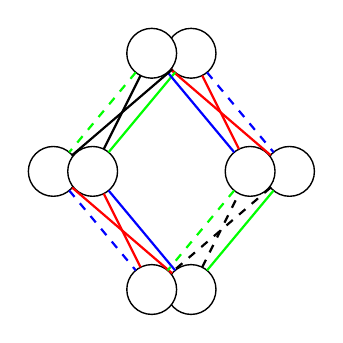
\begin{tikzpicture}[scale=0.05]
\SetVertexNoLabel
\SetUpEdge[labelstyle={draw}]
\Vertex[x=0,y=0]{A}
\Vertex[x=-10,y=0]{H}
\Vertex[x=-35,y=30]{C}
\Vertex[x=-25,y=30]{B}
\Vertex[x=25,y=30]{D}
\Vertex[x=15,y=30]{E}
\Vertex[x=0,y=60]{G}
\Vertex[x=-10,y=60]{F}
\Edge[color=red](A)(C)
\Edge[color=red](B)(H)
\Edge[color=red](G)(E)
\Edge[color=red](F)(D)
\Edge[color=green](A)(D)
\Edge[color=green, style=dashed](E)(H)
\Edge[color=green](G)(B)
\Edge[color=green, style=dashed](F)(C)
\Edge[color=blue, style=dashed](C)(H)
\Edge[color=blue](B)(A)
\Edge[color=blue, style=dashed](G)(D)
\Edge[color=blue](F)(E)
\Edge[color=black, style=dashed](D)(H)
\Edge[color=black, style=dashed](A)(E)
\Edge[color=black](G)(C)
\Edge[color=black](B)(F)
\end{tikzpicture}

\caption{A $2$-d Adinkra with $(2,2)$ colors. The bigrading is visualized by the northwest and northeast directions, respectively (so the two vertices on the left have $h_L = 1$ and $h_R = 0$, for example). \label{fig:2d-example}}
\end{center}
\end{figure}

\section{Structural Theorems}
\label{sec:structural}

In this section, we show that the coherence conditions of $2$-d adinkras force a lot of structure onto them. The main idea is that we can think of the vertices of $2$-d adinkras as arranged in a rectangle, with the stucture of the entire adinkra basically determined by a horizontal and a vertical ``slice'' of the picture.

Let the \emph{support} of a $2$-d adinkra (and/or its bigrading function $(h_L,h_R)$) be defined as the range of $(h_L,h_R)$, its bigrading function. Now, we show that the support of a connected $2$-d adinkra must form a rectangle in $\ZZ^2$.

Let $\sigma$ be a color sequence.  Let $l(\sigma)$ be a rearrangement of $\sigma$ that moves all the left-moving colors to the beginning, and let $r(\sigma)$ be a rearrangement of $\sigma$ that moves all the right-moving colors to the beginning. Thus, suppose $p = q = 2$, we have $l((3,1,2,1)) = (2,1,1,3)$ and $r((3,1,2,1)) = (3,2,1,1)$. We always have $s(l(\sigma)) = s(r(\sigma))$ in general, since $l(\sigma)$ and $r(\sigma)$ are just permutations of each other.

\begin{prop}
\label{prop:reorderpath}
If $v_1$ and $v_2$ are vertices of a $2$-d Adinkra, and $p$ is a path from $v_1$ to $v_2$, then there exists a path $p_L$ consisting only of left-moving edges from $v_1$ to a vertex $u$, and a path $p_R$ consisting only of right-moving edges from $u$ to $v_2$.

Likewise there exists a path $q_R$ consisting only of right-moving edges from $v_1$ to a vertex $w$, and a path $q_L$ consisting only of left-moving edges from $w$ to $v_2$.
\end{prop}

\begin{proof}
Take the color sequence $\sigma$ of the path $p$.  Then $s(\sigma)v_1=v_2$.  Let $\sigma_L$ be the subsequence consisting only of the left-moving colors, and let $\sigma_R$ be the subsequence consisting only of the right-moving colors.  Using Proposition~\ref{prop:colorpath}, we obtain the path $p_L$.  Let $x$ be the endpoint of this path.  We again use Proposition~\ref{prop:colorpath} with $\sigma_R$ starting from $x$, and obtain the path $p_R$.  By Proposition~\ref{prop:colorendpath}, the end of this path is $s(\sigma_R)s(\sigma_L)v_1=s(\sigma_R\sigma_L)v_1=s(\sigma)v_1=v_2$.

The remaining result follows by symmetry.
\end{proof}


\begin{prop}
\label{prop:rectangle-completion}
Let $A$ be a connected Adinkra.  Suppose $(x_1,y_1)$ and $(x_2,y_2)$ are in the support of $A$.  Then $(x_1,y_2)$ and $(x_2,y_1)$ are also in the support of $A$.
\end{prop}
\begin{proof}
The statement that $(x_1,y_1)$ and $(x_2,y_2)$ is in the support of $A$ means that there exist vertices $v_1$ and $v_2$ of $A$ with $(h_L(v_1),h_R(v_1))=(x_1,y_1)$ and $(h_L(v_2),h_R(v_2))=(x_2,y_2)$, respectively.  Since $A$ is connected, there exists a path from $v_1$ to $v_2$.

By Proposition~\ref{prop:reorderpath}, there is a left-moving path from $v_1$ to a vertex $u$ and a right-moving path from $u$ to $v_2$.  Then $h_R(u)=h_R(v_1)=y_1$ and $h_L(u)=h_L(v_2)=x_2$.  Therefore $(x_2,y_1)$ is in the support of $A$.

In the same way, Proposition~\ref{prop:reorderpath} provides a vertex $w$ with bigrading $(x_1,y_2)$.
\end{proof}

\begin{cor}
\label{cor:rectangle}
The support of a connected $2$-d adinkra is a rectangle.  That is, there exist integers $x_0$, $x_1$, $y_0$, and $y_1$ so that the support is
\[\{(x,y)\in\ZZ^2\,|\,x_0\le x\le x_1\mbox{ and }y_0\le y\le y_1\}\]
\end{cor}
\begin{proof}
Let $x_0$ and $y_0$ be the minima of the $x$ and $y$ coordinates, respectively, of the support of the Adinkra.  By Proposition~\ref{prop:rectangle-completion}, $(x_0,y_0)$ is in the support as well.

Likewise, if $x_1$ and $y_1$ are the maxima of the $x$ and $y$ coordinates, respectively, of the support of the Adinkra, then $(x_1,y_1)$ is in the support.  By Proposition~\ref{prop:rectangle-completion}, $(x_1,y_0)$ and $(x_0,y_1)$ are also in the support.

Since the Adinkra is connected, there must be paths from vertices with bigrading $(x_0,y_0)$ to vertices with bigrading $(x_1,y_1)$.  Since $h_L$ and $h_R$ can change by at most 1 along these paths, we see that for all $x_0\le x\le x_1$, there must exist $y_x$ so that $(x,y_x)$ is in the support.  Likewise for all $y_0\le y\le y_1$, there must exist $x_y$ so that $(x_y,y)$ is in the support.  By application of Proposition~\ref{prop:rectangle-completion} again, we get that $(x,y)$ is in the support for all $x_0\le x\le x_1$ and $y_0\le y\le y_1$.
\end{proof}

While it is neat that the vertices of a $2$-d adinkra $A$ line up nicely in a rectangle, we now show that there is even more regularity in its structure. Let $A_L$ (resp. $A_R)$ be the subgraphs of $A$ induced by left-moving (resp. right-moving) edges of $A$. %

\begin{lem}
\label{lem:qiso}
Let $A$ be a $2$-d Adinkra.  If $X$ is a connected component of $A_L$ and $i$ is a right-moving color, then there is a graph isomorphism between $X$ and $q_i(X)$ that preserves colors and $h_L$.  The analogous statement for $A_R$ also holds.
\end{lem}
\begin{proof}
Propostion~\ref{prop:qmap} states that $q_i$ is a graph isomorphism from the underlying graph of $A$ to itself that preserves colors.  If we restrict  $q_i$ to a connected component $X$ of $A_L$, the restricted map is an isomorphism from $X$ to $q_i(X)$ that preserves colors.

Since $i$ is a right-moving color, then for all vertices $v\in X$, $h_L(v)=h_L(q_i(v))$.
\end{proof}

\begin{lem}
\label{lem:qiconnected}
Let $A$ be a $2$-d Adinkra.  If $X$ is a connected component of $A_L$ and $i$ is a right-moving color, then $q_i(X)$ is the vertex set of a connected component of $A_L$. The analogous statement for $A_R$ also holds.
\end{lem}
\begin{proof}
Because the property of connectedness is preserved under graph isomorphism, we know that $q_i(X)$ is connected.  If we let $X'$ be the connected component of $A_L$ that contains $q_i(X)$, then the same argument proves that $q_i(X')$ is connected as well.  Since $X$ was assumed to be a connected component of $A_L$, we have that $q_i(X')\subseteq X$.  But since $q_i^2$ is the identity, $X=q_i^2(X)\subseteq q_i(X')\subseteq X$.  This means $q_i(X')=X$.  By the fact that $q_i^2$ is the identity, we also have $q_i(X)=X'$.
\end{proof}

\begin{prop}
\label{prop:kevin}
Let $A$ be a connected $2$-d Adinkra.  All connected components of $A_L$ (and respectively $A_R$) are isomorphic as graded posets.
\end{prop}
\begin{proof}
Let $X$ and $Y$ be two connected components of $A_L$. Pick vertices $x \in X$ and $y \in Y$. Since $A$ is connected, there is a path from $x$ to $y$ in $A$.  Using Proposition~\ref{prop:reorderpath}, reorder the path so that the right-moving edges occur before the left-moving edges. Since the left-moving edges stay in $Y$, the right-moving edges alone take $x$ to a vertex $y' \in Y$.  The sequence of right-moving edges provides a color sequence $i_1,\ldots,i_k$, and thus, a sequence of compositions $q_{i_k}\circ\cdots\circ q_{i_1}$.  Now $q_{i_k}\circ\cdots\circ q_{i_1}(x)=y'$.  By repeated application of Lemma~\ref{lem:qiconnected}, we have that $q_{i_k}\circ\cdots\circ q_{i_1}(X)$ is a connected component of $A_L$ that contains $y'$, which is $Y$.  By repeated application of Lemma~\ref{lem:qiso}, we have an isomorphism of graphs that preserves colors and the grading $h_L$.
\end{proof}

With all this redundancy, what is the minimal amount of information required for us to understand a $2$-d adinkra? Proposition~\ref{prop:kevin} suggests we just need a single connected component for each direction to give us all the data; this turns out to basically be true, as we see in the upcoming sections.

\section{Products}
\label{sec:products}

Section \ref{sec:structural} hints that the information contained in a $2$-d Adinkra may be captured by just looking at two ``slices'' of the Adinkra. It is natural to guess that there is some product structure lying underneath, especially given the rectangular shape of the support proven in Corollary~\ref{cor:rectangle}. It is also desirable to have some way of combining Adinkras to make bigger ones (and conversely, breaking down bigger ones into smaller pieces). These considerations induce us to consider products of Adinkras. It turns out that one way to get $2$-d Adinkras is to take a product of two $1$-d Adinkras, where the first Adinkra gives the left-moving colors and the second Adinkra gives the right-moving colors. We will eventually see in the next section that this operation (plus a quotient) is all we need to characterize a $2$-d Adinkra.

\begin{construction}
\label{const:product}
Let $p$ and $q$ be non-negative integers.  Let $A_1=(V_1, E_1, c_1, \mu_1,h_1)$ be a $1$-d Adinkra with $p$ colors and let $A_2=(V_2, E_2, c_2, \mu_2,h_2)$ be a $1$-d Adinkra $q$ colors.  We define the \emph{product} of these Adinkras $A_1\times A_2$ as the following 2-Adinkra with $(p,q)$ colors:
\[A_1\times A_2=(V,E,c,\mu,h_L,h_R)\]
where
\begin{eqnarray*}
V&=&V_1\times V_2\\
E&=&E_1\cup E_2\mbox{ where}\\
E_1&=&\{((v_1,w),(v_2,w))\,|\,(v_1, v_2)\in E_1,\mbox{ and } w\in V_2\}\\
E_2&=&\{((v,w_1),(v,w_2))\,|\,v\in V, \mbox{ and }(w_1,w_2)\in E_2\}\\
c((v_1,w),(v_2,w))&=&c_1(v_1,v_2)\mbox{ for all $((v_1,w),(v_2,w))\in E_1$}\\
c((v,w_1),(v,w_2))&=&p+c_2(w_1,w_2)\mbox{ for all $(v,w_1),(v,w_2)\in E_2$}\\
h_L(v,w)&=&h_1(v)\\
h_R(v,w)&=&h_2(w)\\
\mu((v_1,w),(v_2,w))&=&\mu_1(v_1,v_2)\\
\mu((v,w_1),(v,w_2))&=&\mu_2(w_1,w_2)+h_1(v)\pmod{2}
\end{eqnarray*}
See Figure~\ref{fig:product} for an example.
\end{construction}

\begin{figure}
\begin{center}
\begin{tabular}{c|c|c}
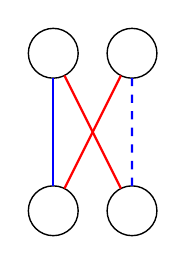
\begin{tikzpicture}[scale=0.1]
%\SetVertexNormal
\SetUpEdge[labelstyle={draw}]
\SetVertexNoLabel
\Vertex[x=0,y=0]{A}
\Vertex[x=10,y=0]{B}
\Vertex[x=0,y=20]{E}
\Vertex[x=10,y=20]{F}
\Edge[color=blue](A)(E)
\Edge[color=blue, style=dashed](B)(F)
\Edge[color=red](A)(F)
\Edge[color=red](B)(E)
\end{tikzpicture}
&
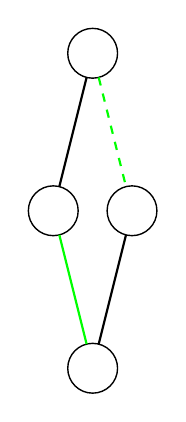
\begin{tikzpicture}[scale=0.1]
\SetVertexNoLabel
\Vertex[x=0,y=0]{A}
\Vertex[x=0,y=40]{B}
\Vertex[x=-5,y=20]{E}
\Vertex[x=5,y=20]{F}
\Edge[color=green](A)(E)
\Edge[color=green, style=dashed](B)(F)
\Edge[color=black](A)(F)
\Edge[color=black](B)(E)
\end{tikzpicture}
&
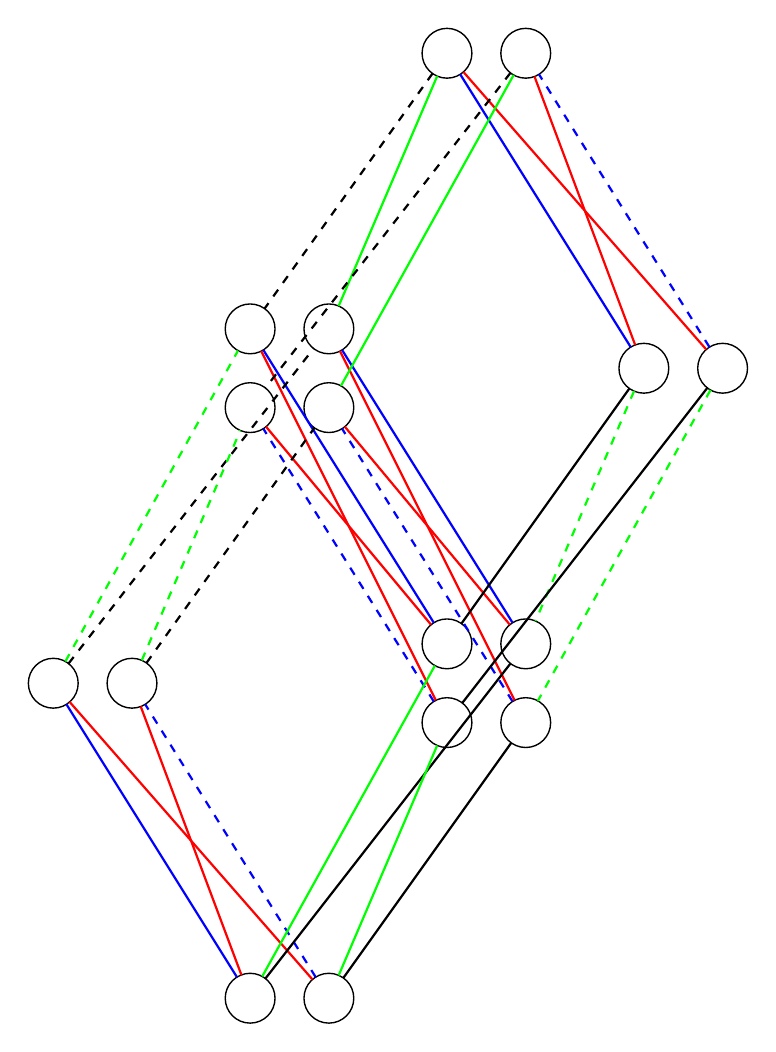
\begin{tikzpicture}[scale=0.1]
%\SetVertexNormal
\SetVertexNoLabel
\SetUpEdge[labelstyle={draw}]
\Vertex[x=0,y=0]{BA}
\Vertex[x=-10,y=0]{AA}
\Vertex[x=-35,y=40]{EA}
\Vertex[x=-25,y=40]{FA}
\Vertex[x=25,y=45]{AF}
\Vertex[x=15,y=45]{AE}
\Vertex[x=0,y=85]{EF}
\Vertex[x=-10,y=85]{EE}
\Vertex[x=0,y=75]{FF}
\Vertex[x=-10,y=75]{FE}

\Vertex[x=40,y=80]{AB}
\Vertex[x=50,y=80]{BB}
\Vertex[x=15,y=120]{EB}
\Vertex[x=25,y=120]{FB}
\Vertex[x=25,y=35]{BF}
\Vertex[x=15,y=35]{BE}

\Edge[color=blue](AA)(EA)
\Edge[color=blue, style=dashed](BA)(FA)
\Edge[color=red](AA)(FA)
\Edge[color=red](BA)(EA)
\Edge[color=blue](AB)(EB)
\Edge[color=blue, style=dashed](BB)(FB)
\Edge[color=red](AB)(FB)
\Edge[color=red](BB)(EB)
\Edge[color=blue](AE)(EE)
\Edge[color=blue, style=dashed](BE)(FE)
\Edge[color=red](AE)(FE)
\Edge[color=red](BE)(EE)
\Edge[color=blue](AF)(EF)
\Edge[color=blue, style=dashed](BF)(FF)
\Edge[color=red](AF)(FF)
\Edge[color=red](BF)(EF)

\Edge[color=green](AA)(AE)
\Edge[color=green, style=dashed](AB)(AF)
\Edge[color=black](AA)(AF)
\Edge[color=black](AB)(AE)
\Edge[color=green](BA)(BE)
\Edge[color=green, style=dashed](BB)(BF)
\Edge[color=black](BA)(BF)
\Edge[color=black](BB)(BE)

\Edge[color=green, style=dashed](EA)(EE)
\Edge[color=green](EB)(EF)
\Edge[color=black, style=dashed](EA)(EF)
\Edge[color=black, style=dashed](EB)(EE)
\Edge[color=green, style=dashed](FA)(FE)
\Edge[color=green](FB)(FF)
\Edge[color=black, style=dashed](FA)(FF)
\Edge[color=black, style=dashed](FB)(FE)

\end{tikzpicture}
\end{tabular}
\caption{Constructing the $2$-d Adinkra from two smaller $1$-d Adinkras. Note that the dashings are all ``consistent'' with the smaller Adinkras, except for the right-moving edges on the upper-left ``boundary'' of the rectangle; these correspond to right-moving edges where the grading corresponding to the first adinkra has height $1$.\label{fig:product}}
\end{center}
\end{figure}

The main non-obvious part of the definition is the dashings. The naive approach, assigning $\mu((v,w_1), (v,w_2)) = \mu(w_1, w_2)$, would fail to give us the odd parity we desire. This situation is analogous to assigning signs in the differential to a double chain complex, such as in Bott and Tu \cite{bott_tu}, where one would have to do a similar symmetry breaking. We now show that this sign-tweaking in fact gives an admissable dashing:

\begin{prop}
\label{prop:product-admissable}
Given Adinkras $A_1$ and $A_2$, $\mu$ is an admissible dashing for $A_1\times A_2$.  That is, given colors $c_1$ and $c_2$, and vertices $v$, $w$, $x$, and $y$ in $A_1\times A_2$, with edges $(v,w)$, $(w,x)$, $(x,y)$, and $(y,v)$ and colors $c(v,w)=c(x,y)=c_1$ and $c(w,x)=c(y,v)=c_2$, we have $\mu(v,w)+\mu(w,x)+\mu(x,y)+\mu(y,v)\equiv 1 \pmod{2}$.
\end{prop}
\begin{proof}
If $c_1$ and $c_2$ are both left-moving colors, then write $v=(v_1,z)$.  Then $w=(w_1,z)$, $x=(x_1,z)$, and $y=(y_1,z)$.  Then we have
\[\mu(v,w)+\mu(w,x)+\mu(x,y)+\mu(y,v)
= \mu_1(v_1,w_1)+\mu_1(w_1,x_1)+\mu_1(x_1,y_1)+\mu_1(y_1,v_1)\]
and the result follows from the fact that $\mu_1$ was an admissible dashing on $A_1$.

If $c_1$ and $c_2$ are both right-moving colors, then write $v=(z,v_2)$.  Then $w=(z,w_2)$, $x=(z,x_2)$, and $y=(z,y_2)$.  Then
\begin{eqnarray*}
&&\mu(v,w)+\mu(w,x)+\mu(x,y)+\mu(y,v)\\
&=& \mu_2(v_1,w_1)+h_1(z)+\mu_2(w_1,x_1)+h_1(z)+\mu_2(x_1,y_1)+h_1(z)+\mu_2(y_1,v_1)+h_1(z)
\end{eqnarray*}
which modulo $2$ is the same as 
\[\mu_2(v_1,w_1)+\mu_2(w_1,x_1)+\mu_2(x_1,y_1)+\mu_2(y_1,v_1).\]
The result follows from the fact that $\mu_2$ was an admissible dashing on $A_2$.


Now if $c_1$ is left-moving and $c_2$ is right-moving, then write $v=(v_1,v_2)$.  Then $w=(w_1,v_2)$, $x=(w_1,x_2)$, and $y=(v_1,x_2)$.  Now note that $v_1$ and $w_1$ are connected by an edge in $A_1$, so $h_1(v_1)$ and $h_1(v_2)$ differ by 1.  In particular, one of these is even and the other is odd.  Without loss of generality, suppose $h_1(v_1)$ is even.  Then $\mu(v,w)=\mu_1(v_1,w_1)$, $\mu(w,x)=\mu_2(v_2,x_2)+1$, $\mu(x,y)=\mu_1(w_1,v_1)$, and $\mu(y,v)=\mu_2(x_2,v_2)$, and we have
\begin{eqnarray*}
&&\mu_(v,w)+\mu(w,x)+\mu(x,y)+\mu(y,v)\\
&=&\mu_1(v_1,w_1)+\mu_2(v_2,x_2)+1+\mu_1(w_1,v_1)+\mu_2(x_2,v_2)\equiv 1\pmod{2}.
\end{eqnarray*}
\end{proof}

We have shown that our definition of product creates a legitimate $2$-d Adinkra from two $1$-d Adinkras. Recall that Adinkras correspond to linear codes; it is natural to expect that the codes of the relevant Adinkras are related nicely.

\begin{definition}[Extending codes]
Let $p$ and $q$ be non-negative integers and let $n=p+q$.  Define $Z_L:\ZZ_2^p\to\ZZ_2^n$ to be the function that appends $q$ zeros, so that for instance, if $p=4$ and $q=3$, then $Z_L(1011)=1011000$.  Likewise, define $Z_R:\ZZ_2^q\to\ZZ_2^n$ to be the function that prepends $p$ zeros.

Define $\pi_L:\ZZ_2^n\to \ZZ_2^p$ to be the function that deletes the last $q$ bits, and $\pi_R:\ZZ_2^n\to \ZZ_2^q$ to be the function that deletes the first $p$ bits.  Note that $\pi_L$ is a left-inverse of $Z_L$ and $\pi_R$ is a left-inverse of $Z_R$.

Our most common use of this notation is as follows: if $C$ is a binary block code of length $p$, we write $Z_L(C)$ for the image under $Z_L$.  Likewise, if $C'$ is a binary block code of length $q$, we write $Z_R(C)$ for the image under $Z_R$.
\end{definition}

\begin{prop}
Let $A_1$ and $A_2$ be as above.  Then
\[C(A_1\times A_2)=Z_L(C(A_1))\oplus Z_R(C(A_2)).\]
\end{prop}
\begin{proof}
Let $(v_1,v_2)\in A_1\times A_2$.  Let $\vec{x}\in \ZZ_2^N$.  We can write $\vec{x}=\vec{x}_1+\vec{x}_2$ where $\vec{x}_1$ is zero in the last $q$ bits and $\vec{x}_2$ is zero in the first $p$ bits.  Now
\[\vec{x}(v_1,v_2)=(\vec{x}_1+\vec{x}_2)(v_1,v_2)=(\vec{x}_1v_1,\vec{x}_2v_2).\]
This means that $\vec{x}(v_1,v_2)=(v_1,v_2)$ if and only if $\vec{x}_1v_1=v_1$ and $\vec{x}_2 v_2=v_2$. So $\vec{x}\in C(A_1\times A_2)$ if and only if $\vec{x}_1\in Z_L(C(A_1))$ and $\vec{x}_2\in Z_R(C(A_2))$.
\end{proof}





\section{Every $2$-d Adinkra is a Quotient}
\label{sec:quotient}

In Section~\ref{sec:products}, we showed that we can construct a $2$-d Adinkra by a product construction of two $1$-d Adinkras, each of which appears on the boundary of the product. In this section, we settle a conjecture of H\"ubsch \cite{hubsch:weaving} by showing that every $2$-d Adinkra is in fact a quotient of the the product of the two $1$-d Adinkras on its lower boundary. Our main result is:

\begin{thm}
\label{thm:quotient}
Let $A$ be a connected $2$-d Adinkra.  Fix a vertex $\overline{0}$ in $A$ and let $A_L^0$ (resp. $A_R^0$) be the connected component of $A_L$ (resp. $A_R$) containing $\overline{0}$. Then the following hold:
\begin{enumerate}
\item[I] There is a binary block code $K$ of length $n$ so that $K\cap Z_L(C(A_L^0))=0$ and $K\cap Z_R(C(A_R^0))=0$, and
\[C(A)=Z_L(C(A_L^0))\oplus Z_R(C(A_R^0))\oplus K;\]
\item[II] there is a graph isomorphism
\begin{equation}
\label{eqn:quotientiso}
A\cong (A_L^0\times A_R^0)/K
\end{equation}
of the underlying graphs that preserves colors and the bigrading;
\item[III] there is a representative $A'$ in the same vertex switching class of $A_L^0\times A_R^0$ whose dashing is invariant under $K$, and the quotient by $K$ gives a dashing that agrees with the dashing on $A$ when compared via the isomorphism given in $(II)$. 
\end{enumerate}
\end{thm}

We first show parts $(I)$ and $(II)$ of this Theorem, starting with the codes. We delay the proof and relevant definitions of $(III)$ to after.

\begin{lem}
\label{lem:cplus}
\[Z_L(C(A_L^0))\oplus Z_R(C(A_R^0)) \subseteq C(A).\]
\end{lem}
\begin{proof}
Let $g\in Z_L(C(A_L^0))$ and $h\in Z_R(C(A_R^0))$.  Then $g\overline{0}=\overline{0}$ because applying $g$ to $\overline{0}$ results in a path that lies completely inside $A_L^0$, and so the fact that $g\overline{0}=\overline{0}$ in $A_L^0$ (since $g\in Z_L(C(A_L^0))$) results in $g\overline{0}=\overline{0}$ in $A$.  Likewise $h\overline{0}=\overline{0}$.  So $(g+h)\overline{0}=g(h(\overline{0}))=\overline{0}$ and $g+h\in C(A)$.
\end{proof}

\begin{proof}[Proof of Theorem~\ref{thm:quotient}, $(I)$ and $(II)$]
From Lemma~\ref{lem:cplus} and basic linear algebra, there exists a vector subspace $K$ of $\ZZ_2^n$ that is a vector space complement of
$Z_L(C(A_L^0))\oplus Z_R(C(A_R^0))$ in $C(A)$.  That is,
\[C(A)=Z_L(C(A_L^0))\oplus Z_R(C(A_R^0))\oplus K.\]



Since $A_L^0\times A_R^0$ is a $1$-d Adinkra, we have, by Proposition~\ref{prop:actioniso}, a color-preserving action of $\ZZ_2^n$ on $A_L^0\times A_R^0$.  Examining the product structure of $A_L^0\times A_R^0$, if we have $\vec{x}\in \ZZ_2^n$, the action is
\[\vec{x}(v_1,v_2)=(\pi_L(\vec{x})v_1,\pi_R(\vec{x})v_2).\]
In particular, if $\vec{x}=Z_L(\vec{x}_L)$, then
\[Z_L(\vec{x}_L)(v_1,v_2)=(\vec{x}_L v_1,v_2)\]
and if $\vec{x}=Z_R(\vec{x}_R)$,
\[Z_R(\vec{x}_R)(v_1,v_2)=(v_1,\vec{x}_R v_2).\]

When this action is restricted to $K$, the action is faithful because $K\cap Z_L(C(A_L^0))\oplus Z_R(C(A_R^0))=0$.  Since $K$ is a subgroup of $C(A)$, which is doubly even, we see that the action of $K$ is distant.  By Proposition~\ref{prop:quotient}, there is a well-defined graph quotient $(A_L^0\times A_R^0)/K$.





Let $v$ be a vertex in $A$, and let $g\in C(A)$.  Then using the color sequence for $g$, we can use Proposition~\ref{prop:colorpath} to obtain a path starting at $v$.  Since $gv=v$, we know that this path ends at $v$.  Use Proposition~\ref{prop:reorderpath} to turn this path into a concatenation of a left-moving path $p_L$ and a right-moving path $p_R$.  The path $p_L$ ends at the vertex $\pi_L(g)v$.  Given that the path $p_R$ is right-moving and connects $\pi_L(g)v$ to $g$, we have that $h_L(\pi_L(g)v)=h_L(v)$.  Given that $p_L$ is left-moving and connects $g$ to $\pi_L(g)v$, we have that $h_R(\pi_L(g)v)=h_R(v)$.

Likewise, $\pi_R(g)v$ has the same bigrading as $v$.

Suppose $(v_1,v_2)\in A_L^0\times A_R^0$ and $g\in C(A)$.  The action of $g$ on $(v_1,v_2)$ gives $g(v_1,v_2)=(\pi_L(g)v_1,\pi_R(g)v_2)$.  Then $h_L(g(v_1,v_2))=h_L(\pi_L(g)v_1)=h_L(v_1)=h_L(v_1,v_2)$.  Likewise, $h_R(g(v_1,v_2))=h_R(v_1,v_2)$.  Therefore the bigrading descends to the quotient.


We now define a graph homomorphism
\[\Phi:A_L^0\times A_R^0 \to A\]
as follows.

Let $(v_1,v_2)\in A_L^0\times A_R^0$.  Then by Proposition~\ref{prop:transitive}, there is a word $\vec{x}_1\in \ZZ_2^p$ so that $\vec{x}_1\overline{0}=v_1$ and a word $\vec{x}_2 \in\ZZ_2^q$ so that $\vec{x}_2\overline{0}=v_2$.  We define $\Phi(v_1,v_2)=(Z_L(\vec{x}_1)+Z_R(\vec{x}_2))\overline{0}$ in $A$.

The $\vec{x}_1$ and $\vec{x}_2$ are defined up to $Z_L(C(A_L^0))$ and $Z_R(C(A_R^0))$, respectively.  Since $Z_L(C(A_L^0))$ and $Z_R(C(A_R^0))$ are subgroups of $C(A)$, we see that the definition of $\Phi(v_1,v_2)$ does not depend on these choices.

But actually by the same argument, for all $g\in C(A)$, $\Phi(g(v_1,v_2))=(v_1,v_2)$.  Therefore $\Phi$ actually descends to the quotient:

\[\tilde{\Phi}:(A_L^0\times A_R^0)/K\to A\]

Suppose $i$ is a color and $(v_1,v_2)\in A_L^0\times A_R^0$ with $v_1=\vec{x}_1\overline{0}$ and $v_2=\vec{x}_2\overline{0}$.  Let $\vec{e}_i$ be the vector that has a single $1$ in the $i$th bit and $0$s elsewhere, so that for all vertices $v$, $\vec{e}v=q_i(v)$.

Then $\vec{e}(v_1,v_2)$ is a vertex connected to $(v_1,v_2)$ in $A_L^0\times A_R^0$ by an edge of color $i$.

Suppose $i$ is a left-moving color.  Then $\vec{e}_i(v_1,v_2)=(q_i(v_1),v_2)$.

\begin{eqnarray*}
\Phi(\vec{e}_i(v_1,v_2))
&=&\Phi(\vec{e}_iv_1,v_2)\\
&=&(Z_L(\vec{x}_1+\vec{e}_i)+Z_R(\vec{x}_2))\overline{0}\\
&=&\vec{e}_i(Z_L(\vec{x}_1)+Z_R(\vec{x}_2))\overline{0}\\
&=&\vec{e}_i\Phi(v_1,v_2)
\end{eqnarray*}
so that $\Phi$ sends every edge of color $i$ to an edge of color $i$.

A similar argument holds if $i$ is a right-moving color.  Therefore $\Phi$, and likewise $\tilde{\Phi}$, are color-preserving homomorphisms of graphs.

Let $(v_1,v_2)\in A_L^0\times A_R^0$.  
\begin{eqnarray*}
h_L(\Phi(v_1,v_2)) &=& h_L((Z_L(\vec{x}_1)+Z_R(\vec{x}_2))\overline{0})\\
 &=& h_L(Z_R(\vec{x}_2)Z_L(\vec{x}_1)\overline{0})\\
\end{eqnarray*}
Since $Z_R(\vec{x}_2)$ follows right-moving colors, this does not affect $h_L$, and so the above is
\[h_L(Z_L(\vec{x}_1)\overline{0}).\]
Since $Z_L(\vec{x}_1)\overline{0}$ in $A$ is the same as $\vec{x}_1\overline{0}$ in $A_L^0$, we have that this is $h(v_1)$.  On the other hand, in $A_L^0\times A_R^0$, this is $h_L(v_1,v_2)$.

Therefore $\Phi$ preserves $h_L$.  The fact that it preserves $h_R$ is proved similarly.



We now show that $\tilde{\Phi}$ is an isomorphism.

To show that $\tilde{\Phi}$ is onto, let $v$ be a vertex in $A$.  Since $A$ is connected, there is a word $\vec{x}\in \ZZ_2^n$ so that $\vec{x}\overline{0}=v$.  Let $v_1=\pi_L(\vec{x})\overline{0}$ in $A_L^0$ and $v_2=\pi_R(\vec{x})\overline{0}$ in $A_R^0$.  Then $\Phi(v_1,v_2)=(Z_L(\pi_L(\vec{x})) + Z_R(\pi_R(\vec{x})))\overline{0} = \vec{x}\overline{0}= v$.

To show that $\tilde{\Phi}$ is one-to-one, suppose $(v_1,v_2)$ and $(v_3,v_4)$ are vertices in $A_L^0\times A_R^0$ and suppose $\Phi(v_1,v_2)=\Phi(v_3,v_4)$.  Define $\vec{x}_1$, $\vec{x}_2$, $\vec{x}_3$, and $\vec{x}_4$ as above, so that $\vec{x}_1\overline{0}=v_1$, and so on.  We then have $(Z_L(\vec{x}_1)+Z_R(\vec{x}_2))\overline{0}=(Z_L(\vec{x}_3) +Z_R(\vec{x}_4))\overline{0}$.  Then $(Z_L(\vec{x}_3-\vec{x}_1)+Z_R(\vec{x_4}-\vec{x}_2))\overline{0}=\overline{0}$, so that if we let $\vec{y}=Z_L(\vec{x}_3-\vec{x}_1)+Z_R(\vec{x_4}-\vec{x}_2)$, then $\vec{y}\in C(A)$ and $\vec{y}(v_1,v_2)=(v_3,v_4)$.

Since $C(A)=Z_L(C(A_L^0))\oplus Z_R(C(A_R^0))\oplus K$, we can write $\vec{y}=\vec{y}_1+\vec{y}_2+\vec{y}_3$ where $\vec{y}_1\in Z_L(C(A_L^0))$, $\vec{y}_2\in Z_R(C(A_R^0))$, and $\vec{y}_3\in K$.
\begin{eqnarray*}
(\vec{y}_1+\vec{y}_2+\vec{y}_3)(v_1,v_2)&=&(v_3,v_4)\\
\vec{y}_3(\pi_L(\vec{y}_1)v_1,\pi_R(\vec{y}_2)v_2)&=&(v_3,v_4)\\
\vec{y}_3(v_1,v_2)&=&(v_3,v_4)
\end{eqnarray*}
This proves that $\tilde{\Phi}$ is one-to-one.


\com{This is awkward notation}
Take the $h_L(v_1,v_2)=h_1(v_1)$ and note that $h_L(\Phi(v_1,v_2))=h_1(v_1)$.  Likewise $h_R(\Phi(v_1,v_2))=h_2(v_2)$.



\end{proof}

Note that $\Phi(v,\overline{0})=v$ on $A_L^0\times\{\overline{0}\}$, and $\Phi(\overline{0},v)=v$ on $\{\overline{0}\}\times A_R^0$.





\begin{comment}




\begin{figure}[htb]
\begin{center}

\begin{tabular}{c|c}
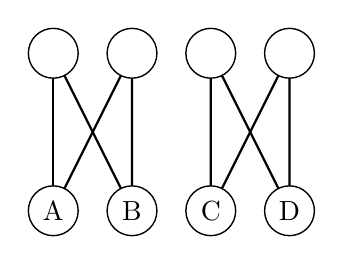
\begin{tikzpicture}[scale=0.10]
%\SetVertexNormal
\SetUpEdge[labelstyle={draw}]
\Vertex[x=0,y=0]{A}
\Vertex[x=10,y=0]{B}
\Vertex[x=20,y=0]{C}
\Vertex[x=30,y=0]{D}
\SetVertexNoLabel
\Vertex[x=0,y=20]{E}
\Vertex[x=10,y=20]{F}
\Vertex[x=20,y=20]{G}
\Vertex[x=30,y=20]{H}
\Edges(A, F, B, E, A)
\Edges(C, H, D, G, C)
\end{tikzpicture}
&
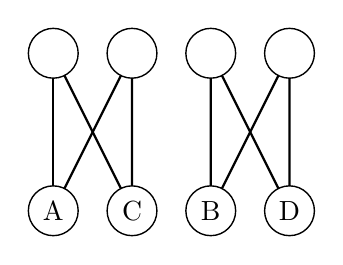
\begin{tikzpicture}[scale=0.10]
%\SetVertexNormal
\SetUpEdge[labelstyle={draw}]
\Vertex[x=0,y=0]{A}
\Vertex[x=10,y=0]{C}
\Vertex[x=20,y=0]{B}
\Vertex[x=30,y=0]{D}
\SetVertexNoLabel
\Vertex[x=0,y=20]{E}
\Vertex[x=10,y=20]{G}
\Vertex[x=20,y=20]{F}
\Vertex[x=30,y=20]{H}
\Edges(A, G, C, E, A)
\Edges(B, H, D, F, B)
\end{tikzpicture}
\end{tabular}
%\includegraphics[scale=0.5]{4cubefold}
\caption{Taking the product of the two adinkras here with the following identification gives a non-disconnected adinkra with 16 vertices. \label{fig:disconnected}}
\end{center}
\end{figure}

\end{comment}

Unfortunately, it is too much to expect the dashing on $A_L^0\times A_R^0$ to agree with the dashing on $A$; it is also almost always false that the dashing on $A_L^0\times A_R^0$ is invariant under the quotienting action of $K$. However, if we allow the operation of \emph{vertex switching}, then we can basically accomplish these goals, giving part $(III)$ of Theorem~\ref{thm:quotient}.

\begin{definition}[Vertex switching]
Given an Adinkra $A$ (either $1$-d or $2$-d), and a vertex $v$ of $A$, we define \emph{vertex switching at $v$} to be the operation on $A$ that returns a new Adinkra $A'$ with the same vertices, edges, coloring, and grading(s) but a new dashing $\mu'$ so that
\begin{equation}
\mu'(e)=\begin{cases}
1-\mu(e),&\mbox{if $e$ is incident to $v$}\\
\mu(e),&\mbox{otherwise.}
\end{cases}
\end{equation}
Vertex switching induces a partition of dashings on $A$ into equivalence classes; call these \emph{vertex switching classes} of $A$.
\end{definition}

\begin{prop}
\label{prop:switching-still-adinkra}
If $A$ is an Adinkra, then so is $A'$.
\end{prop}
\begin{proof}
Since the vertices, edges, coloring, and grading(s) are the same, the only thing to check is the admissibility of $\mu'$.  That is, given colors $c_1$ and $c_2$, and vertices $v$, $w$, $x$, and $y$, such that $(v,w)$ and $(x,y)$ are edges with color $c_1$ and $(w,x)$ and $(y,v)$ are edges with color $c_2$, that $\mu'(v,w)+\mu'(w,x)+\mu'(x,y)+\mu'(y,v)$ is odd.  If $v'$ is none of these vertices, then this sum is unchanged.  If $v'$ is any of these vertices, for instance, $v$, then $\mu'(v,w)$ and $\mu'(y,v)$ are both changed modulo $2$, so that the sum modulo $2$ is still unchanged.
\end{proof}

Douglas, Gates, and Wang \cite{douglas} examined dashings in adinkras from a point of view inspired by Seidel's \emph{two-graphs} \cite{seidel:survey} \footnote{In Seidel's setting, \emph{vertex switching} switched the existence of edges, not the sign of edges; this can be seen as equivalent our definition applied to the complete graph. The type of vertex switching we do in this paper is sometimes called vertex switching on \emph{signed graphs}, to disambiguate from Seidel's usage.}. The second author \cite{zhang:adinkras} enumerated vertex switching classes and the number of dashings of $1$-d Adinkras. In this work, we use vertex switchings again to study $2$-d Adinkras.

Consider the dashing $\mu$ on $A$.  This restricts to $A_L^0$ and $A_R^0$, and Construction~\ref{const:product} produces a dashing $\mu_1$ on $A_L^0\times A_R^0$.   The graph homomorphism
\[\Phi:A_L^0\times A_R^0\to A\]
pulls back the dashing $\mu$ to $\mu_2$ on $A_L^0\times A_R^0$. While $\mu_1$ and $\mu_2$ are fairly different, they agree on the ``lower boundary:''

\begin{lem}
\label{lem:agree-on-boundary}
The dashings $\mu_1$ and $\mu_2$ agree on $A_L^0\times \{\overline{0}\}$ and on $\{\overline{0}\}\times A_R^0$.
\end{lem}
\begin{proof}
The construction of $\mu_1$ gives all edges in $A_L^0\times\{\overline{0}\}$ as the same as in $A_L^0$ under the association of every edge $(v,w)$ with $((v,\overline{0}),(w,\overline{0}))$.  For $\mu_2$, consider that $i_3$ sends every vector $v\in A_L^0$ to $(v,\overline{0})$, and likewise any edges in $A_L^0$ will be sent to the corresponding edge in $A_L^0\times\{\overline{0}\}$.  Therefore $\mu_1$ and $\mu_2$ agree on $A_L^0\times\{\overline{0}\}$.  Likewise for $\{0\}\times A_R^0$.
\end{proof}

Note that part $(III)$ of Theorem~\ref{thm:quotient} can be reformulated as saying that $\mu_1$ and $\mu_2$ are equivalent under vertex switching. Our strategy will be to reduce the problem to checking a set of local conditions on cycles. We now give some definitions and auxiliary results for our approach.


\begin{lem}
\label{lem:cycles-switching-class}
Two dashings have the same parity on all cycles\footnote{This type of result has a natural reformulation with homological algebra, done in independent ways by the first author's work using cubical cohomology \cite{dil:cohomology} and the second author's work using CW-complexes \cite{zhang:adinkras}. In either formulation, having parities of $\mu_1$ and $\mu_2$ agree on cycles is equivalent to $\mu_1 = \mu_2 = 0$ in cohomology.} if and only if they belong to the same vertex switching class.
\end{lem}

\begin{proof}
Let the dashings be $\mu$ and $\mu'$ on the Adinkra $A$. Since vertex switching preserves parity on any cycle, the ``if'' direction is trivial and it suffices to prove the other direction.

Assume $\mu$ and $\mu'$ have the same parity on all cycles. It suffices to prove the statement for $A$ connected, since we can repeat our argument on each connected component of $A$. Pick a spanning tree $T$ of $A$, and pick a vertex $v$ of $A$ to serve as the root. The choice of $v$ induces a map $d$ on the vertices of $A$ that associates to each vertex its distance from $v$ using just edges in $T$ (so $d(v) = 0$), which in turn induces a map on the edges of $T$ by associating to each edge $(x,y)$ the min of $d(x)$ and $d(y)$ (these two values are necessarily $1$ apart). We denote this value $d(x,y)$, which gives a partial ordering on the edges of $T$, which we also call $d$ by slight abuse of notation; to be precise, $d((x,y)) < d((x,y))$ in the ordering $d$ whenever $d(x,y) < d(x,y)$ in the edge function $d$.

Now, extend $d$ to a total ordering $d'$ on the edges of $T$. We claim that we can vertex switch $\mu$ such that $\mu$ agrees with $\mu'$ on $T$. Take the minimal edge $e$ (under $d'$) where the two dashings differ. $e = (x,y)$, where without loss of generality $d(y) > d(x)$. Note that vertex switching at $y$ cannot change the dashing on any of the edges $e < e'$ under the ordering $d'$, since otherwise $d(y)$ should have been assigned a smaller value. Thus, we can greedily vertex switch to make $\mu$ and $\mu'$ equal on $T$.

Finally, if $\mu$ and $\mu'$ are equal on $T$, consider any edge $e$ not in $T$. This edge completes at least one cycle with edges in $T$ (otherwise $T$ was not a minimal spanning tree). Since the two cycles have the same parity in $\mu$ and $\mu'$ by assumption and the dashings agree on all edges but $e$, $e$ must be dashed in the same way under the two dashings. Thus, the two dashings must actually agree on all edges, meaning the two original dashings are in the same vertex switching class.
% However, since $\mu$ and $\mu'$ agree on all cyclesminimal cycles, they agree on all cycles by Lemma~\ref{lem:minimal-cycles-to-all-cycles}, and in particular this cycle. 

\end{proof}

In light of the above Lemma, it suffices for us to prove that the parities of $\mu_1$ and $\mu_2$ agree on all cycles of $A_L^0\times A_R^0$:

\begin{proof}[Proof of Theorem~\ref{thm:quotient}, $(III)$]
Let our cycle be $(v_0,v_1,\ldots,v_k)$ with $v_0=v_k$. We first consider the case where $v_0=\overline{0}$.  Then there is a color sequence $\sigma$ from this.  We modify the path (and thereby modify the color sequence) by ``bubble sorting'' the colors.  Earlier, we noted that we could rearrange $\sigma$ to $l(\sigma)$ so that the left-moving colors were before the right-moving colors.  This can be more specifically done by a series of adjacent swaps of the type that sends the color sequence
\[(i_1,\ldots,i_{j-1},i_j,i_{j+1},i_{j+2},\ldots,i_k)\]
to
\[(i_1,\ldots,i_{j-1},i_{j+1},i_j,i_{j+2},\ldots,i_k).\]
A color swap of this type leads to a new path from $\overline{0}$, via Proposition~\ref{prop:colorpath}.  The path is unchanged up to $v_{j-1}$, but by the definition of Adinkras, property 3, the path returns to $v_{j+1}$ so it is only $v_j$ that has changed.  The effect on the parity of any dashing is, by property 3, to add $1$ modulo $2$.  In particular, $\mu_1$ and $\mu_2$ are both affected in the same way.

After a series of such color swaps, we rearrange $\sigma$ to $l(\sigma)$, and the path in question consists of left-moving edges, which remain in $A_L^0\times \{\overline{0}\}$, and then right-moving edges, which ends in $\overline{0}$, and so must be in $\{\overline{0}\}\times A_R^0$.  By Lemma~\ref{lem:agree-on-boundary}, $\mu_1$ and $\mu_2$ are equal here, and so their parity on this modified path is the same.  Therefore, their parity on the original loop was the same.

Now we consider loops $p$ where $v_0\not=\overline{0}$.  Since $A_L^0\times A_R^0$ is connected, there is a path $p_0$ from $\overline{0}$ to $v_0$.  Take the path $p_0$, followed by $p$, then followed by $p_0^{-1}$ (meaning $p_0$ traversed in the opposite sense).  This is a loop starting and ending in $\overline{0}$, but the parity of a dashing is the same as that of $p$, since every new edge in $p_0$ is counterbalanced by a new edge in $p_0^{-1}$.  Therefore the parity of $\mu_1$ and $\mu_2$ agree on all loops.
\end{proof}

 \com{This is the only place now where we refer to color sequences in any substantial way that is not subsumed by \ref{prop:reorderpath}.}
 
Theorem~\ref{thm:quotient} tells us that our quotient (which did not, a priori, play well with dashing) respects dashing if we allow the action of vertex switching; an alternative interpretation is that dashings should really be thought of as equivalence classes.

\begin{comment} % isn't this already proved?

\begin{lem}
\label{lem:minimal-cycles-to-all-cycles}
The set of parities on all cycles of an Adinkra $A$ are determined by parties on minimal (under inclusion) cycles of $A$.
\end{lem}
\begin{proof}
Consider a cycle in a graph as a $\mathbb{F}_2$-vector space over the edges of the graph. It is easy to check that any cycle $C$ is then a sum (as vectors in this vector space) of minimal cycles $C_1, \ldots, C_k$ and the parity of $C$ under a dashing is the sum of the parities of the minimal cycles $C_i$: each dashed edge in the $C_i$'s either appears twice and thus contributes $0$ to the parity (in which case it was not in $C$) or appears once and thus contributes $1$ to the parity (in which case it was in $C$). 
\end{proof}



\begin{proof}
Thanks to Proposition~\ref{prop:product-admissable}, we know that $\mu_1$ is admissable; we now show that $\mu_2$ is admissable as well. What we must prove is the following: given colors $c_1$ and $c_2$, and vertices $v$, $w$, $x$, and $y$, with edges $(v,w)$, $(w,x)$, $(x,y)$, and $(y,v)$ and colors $c(v,w)=c(x,y)=c_1$ and $c(w,x)=c(y,v)=c_2$, we have $\mu_2(v,w)+\mu_2(w,x)+\mu_2(x,y)+\mu_2(y,v)\equiv 1 \pmod{2}$.

Since $\pi$ is a graph homomorphism, and $c_1$, $c_2$, $v$, $w$, $x$, and $y$ are as above, then $\pi(v)$, $\pi(w)$, $\pi(x)$, and $\pi(y)$ satisfy the same condition.  If $\mu_2=\pi^*(\mu)$, then $\mu_2(v,w)+\mu_2(w,x)+\mu_2(x,y)+\mu_2(y,v)=\mu(\pi(v,w))+\mu(\pi(w,x))+\mu(\pi(x,y))+\mu(\pi(y,v))$ and the result follows from the fact that $\mu$ is an admissible dashing.


\end{proof}
\end{comment}


\section{ESDE Codes}

We have shown that each $2$-d Adinkra is constructed from a pair of $1$-d Adinkras plus a code; it is natural to ask which codes can appear. In this section, we classify these codes, which is another part of the conjectures of H\"ubsch \cite{hubsch:weaving}. 

\begin{definition}[Weights, ESDE codes]
Let $p$ and $q$ be non-negative integers so that $p+q=n$. For any $S \subset [n]$ and every element $\vec{x} \in \ZZ_2^n$, define $\wt_S(\vec{x})$ to be the number of $1$'s in the places corresponding to $S$; so in particular, $\wt_{[n]} = \wt$ as functions. Define an \emph{ESDE (even-split doubly-even) code of length $(p,q)$} to be a doubly-even code of length $n$ and a partition $L \cup R = [n]$ such that $|L| = p$, $|R| = q$, and every word $\vec{x}$ in the code has both $\wt_L(\vec{x})$ and $\wt_R(\vec{x})$ be even-valued. For our work, we always assume that $L = \{1, 2, \ldots, p\}$ and $R = \{p+1, p+2, \ldots, n\}$, since we can permute the indices without changing the structure of the code.
\end{definition}

We remark that ESDE codes are no more restrictive than doubly-even codes; an illustrative example is that any doubly-even code can be made into an ESDE code trivially by assigning $(p,q) = (n, 0)$ or $(0, n)$. This corresponds to the fact that any $1$-d Adinkra is trivially a $2$-d Adinkra with all colors left-moving or all colors right-moving. The main data in ESDE codes is the splitting. In fact, they are quite easy to classify:

\begin{prop}
\label{prop:esde}
Given a doubly-even $[n,k]$-code $C$, there is a bijection between codewords in $C^\perp$ and (ordered) paritions $L \cup R$ that make $C$ into an ESDE. There are $2^{n-k}$ such partitions. 
\end{prop}

\begin{proof}
Consider a partition $L \cup R$ that makes $C$ into an ESDE, and consider the codeword $w$ that is defined to have $1$ at all the positions in $L$ and $0$ at all the positions in $R$. By definition of ESDE codes, all codewords in $C$ have an even number of $1$'s in the support of $w$, which is equivalent to saying that $w$ is orthogonal to all the codewords in $C$. Thus, $w \in C^\perp$. Conversely, for any $w \in C^\perp$, $w$ is orthogonal to all codewords in $C$ and thus give an ESDE. Thus, there is a bijection between the two sets. Note these are ordered partitions; the codeword which has $1$ at all the positions in $R$ and $0$ otherwise would give the same paritition, but in reversed order.
\end{proof}


Recall \com{give citation once Kevin decides which theorems to use} that $1$-d chromotopologies are in bijection with quotients of the Hamming cube $I^n$ by a doubly-even code $K$, so any adinkra $A$ has a well-defined associated code $C(A)$ that is uniquely determined by just the graph structure of the adinkra. Our goal is to show that ESDE codes are exactly the codes that appear for $2$-d adinkras.

In \com{[references]}, there was a class of $1$-d Adinkras that were particularly easy to construct and study, called {\em Valise} Adinkras, whose height function had values in two adjacent integers (usually $0$ and $1$).  By analogy, given a ESDE code, we construct a $2$-d Adinkra called the {\em Valise 2-d Adinkra} that has support in a $2\times 2$ square.


\begin{construction}
\label{cons:valise}
Let $K$ be an ESDE code.  We will describe a construction that provides a $2$-d Adinkra with code $K$, called the {\em Valise 2-d Adinkra}. First, since $K$ is doubly-even, there exists a connected $1$-d Adinkra $A$ with code $C(A) = K$. \com{ [reference: this was a construction somewhere else]} Fix a vertex $\overline{0}$ of $A$. Now every vertex $v$ corresponds to a vector $\vec{v} \pmod{K}$. Define $h_L(v) = \wt_L(\vec{v}) \pmod{2}$ and $h_R(v) = \wt_R(\vec{v}) \pmod{2}$. Note that these functions are well-defined since $K$ is ESDE. $(h_L, h_R)$ gives a bigrading to $A$, making it a $2$-d Adinkra. % Note t, h_R(v)) =    For every vertex $v$ of $A$, pick a path from $\overline{0}$ to $v$.  This produces a color sequence $d$.  Define $h_L(v)$ to be the number $\pmod{2}$ of left-moving colors in $d$ and likewise $h_R(v)$ is the number modulo 2 of right-moving colors in $d$.  These functions are well-defined if every path from $\overline{0}$ to $v$ has the same parity in number of left-moving colors and in number of right-moving colors.  This occurs if and only if every loop starting from $\overline{0}$ has an even number of left-moving colors and an odd number of right-moving colors.  If $K$ is ESDE, then this is the case.
\end{construction}

\begin{figure}[htb]
\begin{center}

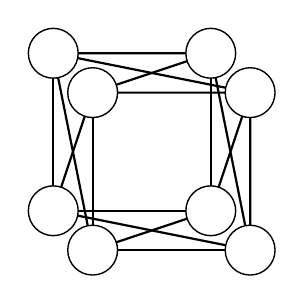
\begin{tikzpicture}[scale=0.10]
%\SetVertexNormal
\SetVertexNoLabel
\SetUpEdge[labelstyle={draw}]
\Vertex[x=0,y=0]{A}
\Vertex[x=-5,y=5]{H}
\Vertex[x=0,y=20]{C}
\Vertex[x=-5,y=25]{B}
\Vertex[x=15,y=5]{D}
\Vertex[x=20,y=0]{E}
\Vertex[x=20,y=20]{G}
\Vertex[x=15,y=25]{F}
\Edges(A,B,G)
\Edges(B,H,C)
\Edges(G,D)
\Edges(C,A,D,H,E,A)
\Edges(D,F,C,G,E,F,B)
\end{tikzpicture}
\caption{A valise $2$-d adinkra that cannot be put into non-valise form.\label{fig:tight valise}}
\end{center}
\end{figure}

\begin{thm}
\label{thm:esde}
For a code $K \subset \ZZ_2^n$, there exists a $2$-d adinkra $A$ with $C(A) = K$ if and only if $K$ is a ESDE code.
\end{thm}
\begin{proof}
Suppose $C(A) = K$ for some $2$-d Adinkra $A$. We know that $K$ is doubly-even. Consider any codeword $\alpha \in K$. Starting at $\overline{0} \in A$, moving by a path corresponding to $\alpha$ must end up back at $\overline{0}$. In particular, it must use an even number of left-moving (resp. right-moving) edges since each of such edge changes the $h_L$ (resp. $h_R$) by $1$ in absolute value. Thus, $C$ must be ESDE. 

Conversely, given an ESDE code $K$, we can use Construction~\ref{cons:valise} to get a $2$-d Adinkra with code $K$. By construction, $A$ is a $1$-d Adinkra with code $K$.  The only thing left to check is whether the $h_L$ and $h_R$ that are defined satisfy the correct properties on edges. Let $(v,w)$ be a left-moving edge in the Adinkra $A$.  Then the color of the edge is left-moving and so $h_L(v)\not=h_L(w)$ and $h_R(v)=h_R(w)$.  Since the possible values for $h_L$ and $h_R$ are $0$ and $1$, it follows that $|h_R(v)-h_R(w)|=1$. The proof is similar for right-moving edges.

\end{proof}

Given a $2$-d Adinkra $A$, with special basepoint $\overline{0}$ and corresponding $A_L^0$ and $A_R^0$, there remains the question of finding the code $K$.  Recall that
\[C(A)=Z_L(C(A_L^0))\oplus Z_R(C(A_R^0))\oplus K.\]
There is some choice involved in defining $K$; it merely has to be a vector space complement to
\[C'=Z_L(C(A_L^0))\oplus Z_R(C(A_R^0)).\]
$K$ will more naturally be defined as $C(A)/C'$, though computationally we can choose a representative to be $K$.


Let $V^0=A_L^0\cap A_R^0$.  Now for every $v\in V^0$, we have $h_L(v)=h_L(\overline{0})$ and $h_R(v)=h_R(\overline{0})$ so in particular, $V^0$ has no edges; only vertices.

We construct a bijection between $V^0$ and $C(A)/C'$.

\begin{construction}
\label{cons:findk}
For every $v\in V^0$, there is a path $p_L$ from $\overline{0}$ to $v$ in $A_L^0$ and a path $p_R$ from $v$ to $\overline{0}$ in $A_R^0$.  These paths give color sequences $\sigma_L$ and $\sigma_R$ with $\beta_L=s(\sigma_L)$ and $\vec{x}_R=s(\sigma_R)$ so that $\vec{x}_L$ is $0$ in the last $q$ coordinates and $\vec{x}_R$ is $0$ in the first $p$ coordinates.  Since the paths $p_L$ and $p_R$ form a loop in $A$, we know that $\vec{x}_L+\vec{x}_R\in C(A)$.

The paths $p_L$ and $p_R$ are not canonical, but if $p'_L$ and $p'_R$ are other paths with those properties, then $p_L(p'_L)^{-1}$ is a loop in $A_L^0$ from $\overline{0}$.  Let $\sigma'_L$ and $\sigma'_R$ be the corresponding color sequences, then $s(\sigma_L)+s(\sigma'_L)\in C(A_L^0)$.  Likewise, $s(\sigma_R)+s(\sigma'_R)\in C(A_R^0)$.

Thus, the choice of $\vec{x}_L+\vec{x}_R$ is well-defined modulo $C'=Z_L(C(A_L^0))\oplus  Z_R(C(A_R^0))$.  This provides a map from $V^0$ to $K=C(A)/C'$.
\end{construction}

\begin{thm}
\label{thm:findk}
The above construction provides a bijective map
\[\Phi:V^0\to C(A)/C'\]
\end{thm}
\begin{proof}

We now prove this map is bijective by providing its inverse.  Suppose $\vec{x}\in C(A)$.  Then by Proposition~\ref{prop:colorpath}, there is a loop in $A$ starting at $\overline{0}$ that follows the colors indicated by $\vec{x}$.  By Proposition~\ref{prop:reorderpath}, there is a left-moving path $p_L$ from $\overline{0}$ to a vertex $v$, and a right-moving path $p_R$ from $v$ to $\overline{0}$.  Since $p_L$ is left-moving, $v\in A_L^0$.  Since $p_R$ is right-moving, $v\in A_R^0$.  Therefore $v\in V^0$.

Note that $v$ does not depend on the order of the left-moving colors in the color sequence, as long as they all come before the right-moving colors.  Thus we have a map
\[\Psi: C(A)  \to V^0.\]

Now suppose $\vec{y}\in Z_L(C(A_L^0))$ and $\vec{z}\in Z_R(C(A_R^0))$.  We consider how the loop in the previous paragraph changes if we replace $\vec{x}$ with $\vec{x}+\vec{y}+\vec{z}$.  We use Proposition~\ref{prop:colorpath} to create a loop $p_1$ in $A_L^0$ that starts at $\overline{0}$ and follows the colors indicated by $\vec{y}$.  Then let $p_2$ be the path from $\overline{0}$ following the colors indicated by $s(\alpha)$ and $p_3$ the path that continues this using $s(\beta)$.  Finally, let $p_4$ be the path from there using the colors of $\vec{z}$.  By Proposition~\ref{prop:colorpath}, since $p_2$ starts from $\overline{0}$, it must still end at the same point $v$.  Therefore the map $\Psi$ descends to a map
\[\tilde{\Psi}:C(A)/C' \to V^0.\]

We now show that this function is the inverse of Construction~\ref{cons:findk}.  Let $v\in V^0$.  The construction gives a path $p_L$ of left-moving edges starting from $\overline{0}$ and ending in $v$ and a path $p_R$ of right-moving edges starting from $v$ to $\overline{0}$.  Composing these paths gives the result of the Construction.  Then we apply $\tilde{\Psi}$.  This takes the code word and finds the loop, which by Proposition~\ref{prop:colorpath} must be $p_Lp_R$.  Then $\Psi$ of the code word is the vertex at the end of $p_L$, which is $v$.

\com{This is a bit messy.  Clean it up}

[show the other composition is the identity]

\end{proof}

\section{Enumerating $2$-d Adinkras}
As a final illustration that we have characterized all $2$-d Adinkras, note that the constructions so far suffice to enumerate all $2$-d Adinkras.

\begin{construction}
First choose an ESDC code $C$.  Let $\pi_L:\ZZ_2^n\to\ZZ_2^p$ and $\pi_R:\ZZ_2^n\to\ZZ_2^q$ be projections onto the first $p$ and last $q$ bits, respectively.

Use the construction from \cite{rAT2} to create the $1$-d Adinkra $A=I^n/C$ with code $C$.  Use the splitting of $[n]$ to designate some edges left-moving and the others, right-moving.  Fix a vertex $\overline{0}$ in $A$.  Let $A_L^0$ and $A_R^0$ be as above. \com{Refer to specific construction}  Use the ``hanging gardens'' construction in Ref.~\cite{hgt} on $A_L^0/\pi_L(C)$ and pull it back to $A_L^0$ to create a height function $h_L$ on $A_L^0$ that is invariant under $\pi_L(C)$.  Likewise create a height function $h_R$ on $A_R^0$ invariant under $\pi_R(C)$.

Now extend $h_L$ on the rest of $A$ as follows: for every vertex $v$ of $A$, pick a path from $\overline{0}$ to $v$.  Use Proposition~\ref{prop:reorderpath} to obtain a left-moving path from $\overline{0}$ to a vertex $w$, and a right-moving path from $w$ to $v$.  Then $w\in A_L^0$ and define $h_L(v)=h_L(w)$.

Likewise define $h_R$ on $A$.
\end{construction}

The fact that the result is a $2$-d Adinkra follows from the following results.

\begin{lem}
The gradings $h_L$ and $h_R$ defined above are independent of the paths $p$ and $q$.\label{lem:indep}
\end{lem}

\begin{proof}
We first prove that $h_L$ is independent of the particular paths $p$ and $q$.  Suppose $p'$ is a left-moving path from $\overline{0}$ to $w'$ and $q'$ is a right-moving path from $w'$ to $v$.  Then $-p$ followed by $p'$ forms a left-moving path from $w$ to $w'$, and $q'$ followed by $-q$ forms a right-moving path from $w'$ to $w$.  These two paths form a cycle and so give an element of $C$.  The left-moving path from $w$ to $w'$ gives an element of $\pi_L(C)$.  Since $h_L$ is invariant under $\pi_L(C)$, we have that $h_L(w)=h_L(w')$.

Therefore $h_L(v)$ is independent of the path chosen.  Likewise $h_R(v)$ is also independent of the path chosen.
\end{proof}

\begin{lem}
If $v$ and $v'$ are vertices and $(v,v')$ is a left-moving edge, then
$|h_L(v)-h_L(v')|=1$ and $h_R(v)=h_R(v')$.  If $(v,v')$ is a right-moving edge, then $|h_R(v)-h_R(v')|=1$ and $h_L(v)=h_L(v')$.
\end{lem}

\begin{proof}
Let $v$ and $v'$ be vertices connected by an edge.  Fix a left-moving path $p$ from $\overline{0}$ to a vertex $w$ in $A_L^0$ and a right-moving path $q$ from $w$ to $v$.  Then $h_L(v)=h_L(w)$.

Suppose the edge $(v,v')$ is a right-moving edge.  By appending to $q$ the edge $(v,v')$, we have a right-moving path from $w$ to $v'$.  By Lemma~\ref{lem:indep}, we have $h_L(v)=h_L(v')$.

Now suppose the edge $(v,v')$ is a left-moving edge.  Let the color of this edge be $i$.  Let $w'=q_i(w)$.  The map $q_i$ is a graph isomorphism that sends the path $q$ to a new right-moving path $q'$ that connects $w'$ to $v'$.

Since there is a left-moving path from $\overline{0}$ to $w'$ (consisting of $p$ appended with an $i$-colored edge) and a right-moving path from $w'$ to $v'$, we know that $h_L(w')=h_L(v')$.  

Since there is a left-moving edge between $w$ and $w'$, we have $|h_L(w)-h_L(w')|=1$.  Since $h_L(w')=h_L(v')$ and $h_L(w)=h_L(v)$, we conclude that $|h_L(v)-h_L(v')|=1$.

The other cases can be obtained by symmetry.
\end{proof}


\begin{thm}
Every $2$-d Adinkra can obtained by this construction.
\end{thm}

\begin{proof}
Given any $2$-d Adinkra $A$, there is an ESDC code $C$.  Pick a vertex $\overline{0}$ and define $A_L^0$ and $A_R^0$ as in (\ref{thm}).

Restrict the gradings $h_L$ and $h_R$ onto $A_L^0$ and $A_R^0$.  Note that if $g\in C$, then $\pi_L(g)v=\pi_R(g)v$, and so $h_L(\pi_L(g)v)=h_L(v)$ and $h_R(\pi_L(g)v)=h_R(v)$.  Therefore $h_L$ restricted to $A_L^0$ is invariant under $\pi_L$.  Likewise $h_R$ restricted to $A_R^0$ is invariant under $\pi_R$.

The dashings, as described in \cite{rAT2}, can be obtained by choosing the specific quotient $I^n/C$.

Theorem~\ref{thm:main} gives a description of $A$ in terms of this construction.

\end{proof}


\section*{Acknowledgments}

The authors wish to thank Charles Doran, Sylvester Gates, and Tristan H\"ubsch for helpful conversation.

\appendix

\section{Representations of supersymmetry}
The $1$-d $n$-extended supersymmetry algebra is a superalgebra consisting of an even operator $H$ and $n$ odd operators $Q_1, \ldots, Q_n$ with the following relations:
\begin{eqnarray}
\label{eqn:susy1d1}
[H,Q_i]&=&0\\
\label{eqn:susy1d2}
\{Q_i,Q_j\}&=&2\delta_{ij}H
\end{eqnarray}

\begin{construction}
\label{cons:susy1d}
Given a $1$-d Adinkra $A=(V,E,c,\mu,h)$ with $n$ colors, we can find a representation $R(A)$ of the $1$-d $n$-extended supersymmetry algebra as follows:
\begin{itemize}
\item Let $R_0$ be the real vector space generated by $V$.  That is, $R_0$ is the set $\{f:V\to \RR\}$ viewed as a vector space with function addition and scalar multiplication.  There is a basis given by $\{b_v\,|\,v\in V\}$ with $b_v(v)=1$ and $b_v(w)=0$ if $v\not=w$.
\item Let $R(A)=R_0\otimes_\RR \RR[H]$.  This is a representation of $\RR[H]$ with $H(b\otimes H^k)=b\otimes H^{k+1}$, and $H$ extends to all of $R$ linearly.
\item If $v\in V$ and $w=q_i(v)$, then
\[Q_i(b_v\otimes H^k)=(-1)^{\mu(v,w)} b_w\otimes H^{k+\frac12(1-h(w)+h(v))}\]
Extend $Q_i$ to all of $R(A)$ linearly.
\item There is a $\ZZ_2$ grading of $R(A)$: let the $\ZZ_2$ grading of $b_v\otimes H^k$ be $h(v)\pmod{2}$.
\end{itemize}
\end{construction}
Note that the exponent of $H$, $i+\frac12(1-h(w)+h(v))$, is an integer because $|h(w)-h(v)|=1$.

\begin{prop}
\label{prop:rep1}
$R$ is a representation of the $1$-d supersymmetry algebra.
\end{prop}
\begin{proof}
First note that each $Q_i$ acts by changing the $\ZZ_2$ grading and $H$ does not.  Therefore the $Q_i$ are odd operators and $H$ is an even operator.

Since $b_v$ is a basis for $R_0$, $b_v\otimes 1$ is a generator of $R$ as an $\RR[H]$-module.  It suffices, then, to prove (\ref{eqn:susy1d1})--(\ref{eqn:susy1d2}) for $b_v\otimes 1$.

If $q_i(v)=w$, then
\begin{eqnarray*}
Q_i(H(b_v\otimes H^k))&=&Q_i(b_v\otimes H^{k+1})\\
&=&(-1)^{\mu(v,w)}b_w\otimes H^{k+1+\frac12(1-h(w)+h(v))}\\
&=&H((-1)^{\mu(v,w)}b_w\otimes H^{k+\frac12(1-h(w)+h(v))})\\
&=&H(Q_i(b_v\otimes H^k))
\end{eqnarray*}

We also have
\begin{eqnarray*}
Q_i(Q_i(b_v\otimes H^k))
&=&Q_i((-1)^{\mu(v,w)} b_w\otimes H^{k+\frac12(1-h(w)+h(v))})\\
&=&(-1)^{\mu(v,w)} (-1)^{\mu(w,v)} b_v\otimes H^{k+\frac12(1-h(w)+h(v))+\frac12(1-h(v)+h(w))}\\
&=&b_v\otimes H^{k+1}\\
&=&H(b_v\otimes H^{k})
\end{eqnarray*}

Now consider $\{Q_i,Q_j\}$ where $i\not=j$.  Let $w=q_i(v)$ and $x=q_j(w)$ and $y=q_i(x)$.  Then from Property 3 of Adinkras, $v=q_j(y)$.
\begin{eqnarray*}
Q_i(Q_j(b_v\otimes H^k))
&=&Q_i((-1)^{\mu(v,y)}b_y\otimes H^{k+\frac12(1-h(y)+h(v))})\\
&=&(-1)^{\mu(v,y)+\mu(y,x)}b_x\otimes H^{k+\frac12(1-h(y)+h(v))+\frac12(1-h(x)+h(y))})\\
&=&(-1)^{\mu(v,y)+\mu(y,x)}b_x\otimes H^{k+\frac12(2-h(x)+h(v))})
\end{eqnarray*}
while
\begin{eqnarray*}
Q_j(Q_i(b_v\otimes H^k))
&=&Q_j((-1)^{\mu(v,w)}b_w\otimes H^{k+\frac12(1-h(w)+h(v))})\\
&=&(-1)^{\mu(v,w)+\mu(w,x)}b_x\otimes H^{k+\frac12(1-h(w)+h(v))+\frac12(1-h(x)+h(w))})\\
&=&(-1)^{\mu(v,w)+\mu(w,x)}b_x\otimes H^{k+\frac12(2-h(x)+h(v))})
\end{eqnarray*}
Since
\[\mu(v,w)+\mu(w,x)+\mu(x,y)+\mu(y,v)\equiv 2\pmod{2},\]
we have
\[Q_jQ_i(b_v\otimes H^k)=-Q_iQ_j(b_v\otimes H^k).\]
\end{proof}

\begin{definition}[Adinkraic representations]
A representation $M$ of $1$-d $n$-extended supersymmetry algebra is called \emph{adinkraic} if there exists a $1$-d Adinkra $A$ with $n$ colors so that $R(A)=M$ in Construction~\ref{cons:susy1d}.
\end{definition}

Though not relevant for our theorems, one can notice that the grading $h$ provides a grading to $R$ in the following way: the mass dimension of $b_v\otimes H^k$ is $k+\frac12 h(v)$.  Then $H$ has grading $1$ and each $Q_i$ has grading $\frac12$.

\subsection{Representations of $2$-d supersymmetry}
The $2$-d $(p,q)$-extended supersymmetry algebra has two even operators $H$ and $P$, and $n$ odd operators $Q_1,\ldots, Q_n$, with the first $p$ being viewed as ``left-moving'' and the remaining $q=n-p$ being viewed as ``right-moving''.  $H$ and $P$ commute with everything, while
\[
\{Q_i, Q_j\}=\begin{cases}
2\delta_{ij}(H+ P),&\mbox{ if $i\le p$}\\
2\delta_{ij}(H- P),&\mbox{ if $i> p$}\\
\end{cases}
\]
We define $P_- = H+ P$ and $P_+=H-P$.

\begin{construction}
Given a $2$-d Adinkra $A=(V,E,c,\mu,h_L,h_R)$ with $(p,q)$ colors, we get a representation of the $2$-d $(p,q)$-extended supersymmetry algebra as follows:
\begin{itemize}
\item Let $R_0=\{f:V\to\RR\}$ as a vector space.  Again, for every $v\in V$ define $b_v(v)=1$ and $b_v(w)=0$ if $v\not=w$.
\item Let $R(A)=R_0\otimes_\RR \RR[P_-,P_+]$ as a free $\RR[P_-,P_+]$-module.
\item If $i\le p$, and $w=q_i(v)$, then define
\[Q_i(b_v\otimes P_-^k P_+^l)=
(-1)^{\mu(v,w)}b_w\otimes P_-^{k+\frac12(1-h_L(w)+h_L(v))}P_+^l \]
\item If $i>p$ then
\[Q_i(b_v\otimes P_-^k P_+^l)=
(-1)^{\mu(v,w)}b_w\otimes P_-^k P_+^{l+\frac12(1-h_L(w)+h_L(v))} \]
\item There is a $\ZZ_2$ grading of $R(A)$: let the $\ZZ_2$ grading of $b_v\otimes H^k$ be $h_L(v)+h_R(v)\pmod{2}$.
\end{itemize}
\end{construction}

\begin{prop}
\label{prop:rep2}
$R(A)$ is a representation of the $2$-d $(p,q)$-extended supersymmetry algebra.
\end{prop}
\begin{proof}
The proof is largely the same as Proposition~\ref{prop:rep1}.
\end{proof}

\begin{construction}
Let $R_L$ be a representation of $1$-d $p$-extended supersymmetry and $R_R$ be a representation of $1$-d $q$-extended supersymmetry.  Then we define
\[R_L\otimes R_R\]
a representation of $2$-d $(p,q)$ supersymmetry as follows.
\begin{itemize}
\item For $i\le p$, $Q_i(a\otimes b)=Q_i(a)\otimes b$.
\item For $i>p$, $Q_i(a\otimes b)=(-1)^{|a|}a\otimes Q_{i-p} b$.
\item $H(a\otimes b)=H a\otimes b + a\otimes Hb$
\item $P(a\otimes b)=Pa \otimes b + a\otimes Pb$
\end{itemize}
Here $|a|$ means the $\ZZ_2$ grading of the element $a$ in $R_L$.
\end{construction}

\begin{prop}
$R_L\otimes R_R$ is a representation of $2$-d $(p,q)$-extended supersymmetry.
\end{prop}
\begin{proof}
This is standard in the SUSY literature.
\end{proof}

\begin{prop}
Let $A_L$ and $A_R$ be $1$-d Adinkras with $p$ and $q$ colors respectively.  Let $R(A_L)$ and $R(A_R)$ be the representations of $1$-d supersymmetry obtained from $A_L$ and $A_R$, respectively, by Construction~\ref{cons:susy1d}.  Then there is an isomorphism of representations of $2$-d $(p,q)$-extended supersymmetry
\[R(A_L)\otimes R(A_R) \cong R(A_L\times A_R)\]
\end{prop}
\begin{proof}
Let $v\in A_L$ and $w\in A_R$.  The isomorphism sends $(b_v\otimes H^k)\otimes (b_w\otimes H^l)$ to $b_{(v,w)}\otimes P_-^{k}P_+^l$.
\end{proof}

\begin{prop}
Let $A$ be an Adinkra and let $v$ be a vertex of $A$.  Let $A'$ be the Adinkra obtained by doing a vertex flip on $v$.  Then there is an isomorphism from $R(A)$ and $R(A')$.
\end{prop}
\begin{proof}
Let $\Phi$ be the linear map that sends $b_v\otimes H^k$ to $-b_v\otimes H^k$, and for every $w\not=v$, $b_w\otimes H^k$ to $b_w\otimes H^k$.

Let $w=q_i(v)$.  Now $Q_i(\Phi(b_v\otimes H^k))=Q_i(-b_v\otimes H^k)=-(-1)^{\mu(v,w)}b_w H^{k+\frac12(1-h(w)+h(v)}=(-1)^{\mu'(v,w)}b_w H^{k+\frac12(1-h(w)+h(v)}=\Phi(Q_i(b_v\otimes H^k))$.

etc. etc. [This is tedious.]
\end{proof}

\begin{prop}
Let $A=(V,E,c,\mu,h_L,h_R)$ and $A'=(V,E,c,\mu,h_L,h_R)$ be $2$-d Adinkras and let $f:V\to V'$ be a graph homomorphism that preserves coloring, dashing, and gradings.  Then the linear map
\[f_*:R(A)\to R(A')\]
\[f_*(b_v\otimes P_-^kP_+^l)=b_{f(v)}\otimes P_-^kP_+^l\]
is a homomorphism of representations.
\end{prop}
\begin{proof}
The map $f_*$ commutes with $P_+$ and $P_-$.  If $i$ is a left-moving color and $q_i(v)=w$, then $q_i(f(v))=f(w)$ and
\[f_*(Q_i(b_v\otimes P_-^kP_+^l))=f_*((-1)^{\mu(v,w)}b_w\otimes P_-^{k+\frac12(1-h_L(w)+h_L(v))}P_+^l\]
while
\[Q_i(f_*(b_v\otimes P_-^kP_+^l))=Q_i(b_{v'}\otimes P_-^kP_+^l)
=(-1)^{\mu'(f(v),f(w))}b_{f(w)}\otimes P_-^{1-h'_L(f(w))-h'_R(f(v))}P_+^l\]
which is the same thing if $f$ preserves dashing and gradings.

Likewise if $i$ is a right-moving color.
\end{proof}

\begin{thm}
If $A$ is a $2$-d Adinkra with $(p,q)$ colors, then 
\[R(A)=(R(A_L^0)\otimes R(A_R^0))/M\]
where $M$ is a submodule.
\end{thm}
\begin{proof}
From the main theorem Theorem~\ref{thm:quotient},
\[A=(A_L^0\times A_R^0)/K\]
and in particular there is a graph homomorphism
\[f:A_L^0\times A_R^0\to A\]
that is surjective and preserves coloring, dashing, and gradings.  Take the coresponding linear map
\[f_*:R(A_L^0\times A_R^0)\to R(A)\]
and let $M$ be the kernel of this map.  Composed with the isomorphism
\[R(A_L^0)\otimes R(A_R^0)\cong R(A_L^0\times A_R^0)\]
we have the isomorphism.
\end{proof}


\section{Equivalence with other notions of $2$-d Adinkras}


If I read Tristan's stuff right, we can completely translate the combinatorial rules to: a \emph{2-d adinkra} (of dimension $n$) is a finite simple connected graph $A$ such that:
\begin{itemize}
\item It is an $1$-d adinkra (with the associated ranking, dashing, etc.).
\item It has $p + q = n$ colors, where the first $p$-colors are called ``left-moving'' and the second $q$-colors are called ``right-moving.''
\item A coherence condition: for any cycle, we imagine the following sum: going up (here ``up'' comes from the grading we have from the engineering dimension in our ranking for the $1$-d adinkra) a left-handed edge adds $-1$, and going up a right-handed edge adds $1$; going down the edges give contributions with opposite signs. The sum of this around any cycle must be $0$. (in particular, this rules out things like ambidextrous bow-ties)
\end{itemize} 

Assuming I interpreted these rules correctly, now I can do combinatorics without needing any physics.

%%

The first structural fact we can impose is a bi-grading that is compatible with the grading we already have from the $1$-d adinkra structure, in the sense that the $1$-d grading is simply one of the coordinates of our bi-grading.

\begin{prop}
A $1$-d adinkra can be extended to a $2$-d adinkra if and only if the $1$-d adinkra has a \emph{bigrading} to $\ZZ^2$. This is a map $g: V \rightarrow \ZZ^2$, such that all left-moving edges correspond to displacements of $(0, 1)$ and right-moving edges correspond to displacements of $(1, 0)$.
\end{prop}

\begin{proof}
Proof delayed until talking more with Kevin and Tristan about the easiest way to write things up to avoid reinventing wheels.
\end{proof}

\bibliographystyle{abbrv}
\bibliography{Adinkras}





\end{document}